\documentclass[conference]{IEEEtran}
\IEEEoverridecommandlockouts

\usepackage{amsmath,amssymb}
\usepackage{booktabs}
\usepackage{multirow}
\usepackage{array}
\usepackage{cite}
\usepackage{url}
\usepackage{graphicx}
\usepackage{xcolor}
\graphicspath{{figures/}}

\newcommand{\wrap}{\operatorname{wrap}}
\newcommand{\Dp}{D_{p}}
\newcommand{\Dtheta}{D_{\theta}}
\newcommand{\Dv}{D_{v}}
\newcommand{\Domega}{D_{\omega}}
\newcommand{\Iomega}{I_{\omega}}

\title{Sensor-Lightweight Digital Twin Fidelity for Mobile Robots Under Changing Conditions:\\
Frozen Evaluation, Physical--Virtual Fidelity, and UGV01 Instantiation}

\author{\IEEEauthorblockN{Shreyas Udaya}
\IEEEauthorblockA{Bradley Department of Electrical and Computer Engineering\\
Virginia Tech\\
Blacksburg, VA, USA\\
\textit{Research status draft --- August 2026}}}

\begin{document}
\maketitle

\begin{abstract}
A digital twin (DT) is more than a generic model of a class of systems: it is a synchronized virtual representation of a particular physical asset at a specified fidelity. For mobile robots, however, fidelity is often reported only through a single localization score. This paper instead studies \emph{physical--virtual synchronization itself}: how a sensor-lightweight computational replica remains faithful, when local agreement fails to preserve long-horizon synchronization, and how much asset-specific calibration is required before a generic model can defensibly be called a twin of one robot. We define a multidimensional fidelity profile containing position, heading, velocity, yaw-rate, finite-horizon, accumulated, percentile, and worst-case divergence. The evaluation is frozen and sequence-aware: 10 held-out i2Nav physical sequences with three seeds, an official benchmark layer, and an AprilTag-referenced UGV01 instantiation. Across i2Nav, Twin V2 reduces ATE RMSE from 2.834 to 2.398~m (15.4\%), heading MAE from 3.336 to 2.569$^{\circ}$ (23.0\%), and RPE$_{10}$ from 0.271 to 0.253~m (6.7\%) relative to Twin V1, while preserving RPE$_1$. Mechanistic analysis shows that low short-horizon RPE can coexist with severe global divergence: \texttt{parking02} has RPE$_{10}=0.097$~m but $Dp$ p95 $=22.345$~m. The benign envelope generalizes strongly for rate-domain disagreement but is sequence-sensitive for global position and heading. On the tracked UGV01, asset-specific calibration reduces same-window ATE from 0.131 to 0.099~m and heading MAE from 13.3 to 5.6$^{\circ}$; the full repaired low-speed carpet result is ATE $=0.114$~m and heading MAE $=6.7^{\circ}$. These results support a condition-dependent fidelity framework, not a claim of universal odometry superiority. The paper closes with the limitations of the current UGV01 condition and the requirements for an untouched synchronized repeat.
\end{abstract}

\begin{IEEEkeywords}
digital twin, mobile robot, fidelity, physical--virtual synchronization, sensor-lightweight systems, cyber-physical systems, trust, wheel-inertial sensing
\end{IEEEkeywords}

\section{Introduction}
Digital twins are increasingly used to connect physical assets with computational representations for monitoring, prediction, control, verification, and cyber-physical decision making. A useful distinction is that a DT is not merely a simulation or generic system model. The Digital Twin Consortium defines a DT around an integrated virtual representation with synchronized interaction at a specified frequency and fidelity~\cite{dtc_definition}. Jones \emph{et al.} similarly identify physical and virtual entities, state, twinning, metrology, and levels of fidelity as central DT characteristics and open research concerns~\cite{jones2020dt}. This distinction is especially important for mobile robots: a generic kinematic or learned motion model may describe a robot class, but it becomes the twin of a particular robot only when it is sufficiently bound to, synchronized with, and validated against that physical asset.

Mobile robots create a difficult DT setting because the physical--virtual relationship changes with wheel slip, surface properties, turning dynamics, actuator response, geometric uncertainty, encoder behavior, inertial bias, timing, and other operating conditions. Heavy perception stacks based on cameras, LiDAR, radar, or GNSS can provide accurate state estimates, but they also increase sensing, bandwidth, compute, power, calibration, and deployment burden. This motivates a sensor-lightweight twin in which wheel/odometry and IMU information are used to maintain a computational replica. The central scientific question is not whether a particular neural network can reduce pose error, but whether the resulting virtual counterpart remains a faithful surrogate of the specific physical robot and whether the limits of that fidelity can be characterized.

The distinction from learned odometry is therefore substantive. Odometry asks how accurately the state of the robot can be estimated. In the present work, trajectory errors are measurements of a broader DT property: \emph{physical--virtual fidelity}. We are concerned with whether the virtual asset remains synchronized with the physical asset across time and operating regimes, why the two diverge, how divergence accumulates, how reproducible that relationship is, how much asset-specific information is required to instantiate the twin, and whether benign divergence is sufficiently bounded for the twin to serve as a trustworthy cyber-physical reference.

\subsection{Problem Statement}
The research problem is:

\begin{quote}
\textbf{How can a sensor-lightweight computational replica of a specific mobile robot be instantiated and maintained as a faithful digital twin, and how can its physical--virtual fidelity, divergence, and trustworthiness be quantified as operating conditions and sensor behavior change?}
\end{quote}

This problem has three coupled dimensions. First, \emph{asset-specific instantiation} asks when a generic model or twin template becomes representative of a particular robot. Second, \emph{fidelity maintenance} asks how well the virtual state tracks the physical state over instantaneous, finite, and long horizons. Third, \emph{trust characterization} asks how much disagreement is expected under benign operation before the twin can be used as a dependable monitoring or security reference.

\subsection{Research Questions}
The current study is organized around the following research questions:
\begin{itemize}
    \item \textbf{RQ1: Fidelity definition.} How should physical--virtual fidelity of a sensor-lightweight mobile-robot DT be defined and quantified without collapsing incompatible quantities such as meters, radians, and sensor residuals into an arbitrary scalar?
    \item \textbf{RQ2: Divergence mechanisms.} Which sensor, dynamics, and operating-condition mismatches dominate benign twin divergence, and why can finite-horizon fidelity remain high while long-horizon synchronization fails?
    \item \textbf{RQ3: Fidelity maintenance and instantiation.} How much asset-specific calibration and sensor information is required for a lightweight twin to maintain bounded fidelity across unseen trajectories and conditions?
    \item \textbf{RQ4: Trust.} What empirical benign divergence envelope characterizes a correctly functioning twin, and how stable is that envelope across sequences, seeds, and operating regimes?
\end{itemize}

\subsection{Intended Contributions}
Because this manuscript is a research-status draft, the contributions below are separated into established evidence and intended final contributions.
\begin{enumerate}
    \item \textbf{A mobile-robot DT fidelity framework.} We formulate fidelity as a multidimensional physical--virtual divergence process and a run-level Twin Fidelity Profile that distinguishes instantaneous state mismatch, finite-horizon relative fidelity, persistent model/sensor bias, accumulated divergence, percentile/worst-case behavior, and sequence-aware variability without collapsing incompatible physical quantities into a single score.
    \item \textbf{A sensor-lightweight twin-maintenance methodology.} We use proprioceptive wheel/odometry and IMU information, a nominal physics model, and bounded learned residual mechanisms to maintain the virtual counterpart without camera, LiDAR, radar, or GNSS input to the learned twin-maintenance model.
    \item \textbf{Mechanistic diagnosis of twin divergence.} We show, using residual and oracle analyses, that a small persistent yaw mismatch can produce severe long-horizon physical--virtual divergence even when 1--10~s relative errors remain small.
    \item \textbf{Condition- and asset-specific trust characterization.} The final study will quantify how fidelity changes with operating conditions and calibration burden, and will establish a benign divergence envelope that can later support cyber-physical fault or attack detection.
    \item \textbf{A sensing--fidelity tradeoff.} The final evaluation will place the lightweight twin relative to heavier sensing systems using compatible official benchmark metrics and, where defensible, sensing/compute burden.
\end{enumerate}

\section{Related Work}
\subsection{Digital Twin Definition and Fidelity}
A large DT literature exists, but the meaning of fidelity is not uniform. Jones \emph{et al.} reviewed 92 DT publications and identified levels of fidelity as one of the important gaps in the field~\cite{jones2020dt}. Kober \emph{et al.} define DT fidelity in terms of how precisely a virtual representation mirrors physical reality and propose an objective-dependent method for selecting an optimum fidelity level in manufacturing~\cite{kober2023fidelity}. More recently, Zhang \emph{et al.} proposed a quantitative fidelity-evaluation method for aero-engine assembly DTs, separating fidelity into multiple dimensions and studying fidelity evolution across an assembly process~\cite{zhang2025fidelity}. These works establish that fidelity is a first-class DT property rather than merely a model-accuracy statistic. However, they do not address the specific problem of a mobile asset whose physical--virtual error evolves continuously under slip, turning, sensor bias, and trajectory-dependent motion.

The present work adopts the DT principle that synchronization and fidelity must be validated for the particular physical asset~\cite{dtc_definition}. We therefore avoid calling an unadapted generic cross-platform model a DT of a new robot. Instead, such a model is treated as a \emph{twin template}; asset-specific calibration or adaptation instantiates the template for a particular physical platform.

\subsection{Digital Twins for Mobile Robots and Physical--Virtual Synchronization}
Digital-twin methods have been applied directly to mobile robots. Ding \emph{et al.} introduced Robopheus, a virtual--physical interactive mobile-robot testbed that dynamically learns models from the physical environment and reported substantially improved physical trajectory accuracy through virtual--physical interaction~\cite{ding2021robopheus}. Yang \emph{et al.} developed a DT-based navigation and control system for an omnidirectional mobile robot and reported a 0.061~m physical--virtual synchronization tracking error using synchronization control~\cite{yang2025omr}. Betzer \emph{et al.} used a DT as a cloud-based watchdog for runtime verification of a TurtleBot under uncertainty and reported up to a 41\% reduction in the difference between actual and expected speeds~\cite{betzer2024runtime}.

These studies demonstrate that physical--virtual synchronization can improve control or support runtime verification. Our focus is complementary but different: we study the \emph{fidelity of the twin itself as the primary object}, including its dependence on sensing, persistent model error, operating regime, asset-specific instantiation, seed/sequence variability, and benign divergence bounds. In particular, we do not assume that a DT used as a monitor is already sufficiently faithful; we attempt to quantify when that assumption is justified.

\subsection{Wheel--Inertial Odometry as an Enabling Technology}
The closest robotics literature is wheel--inertial state estimation. WING uses IMU and wheel encoders, neural correction, uncertainty modeling, and a continuous ground-manifold constraint to obtain accurate interoceptive-only odometry~\cite{jiang2025wing}. This is highly relevant because it demonstrates the performance achievable using lightweight proprioceptive sensing. However, the primary objective of WING is pose/state estimation. Our work uses related sensing and motion-correction concepts as mechanisms inside a DT, but evaluates a different system property: asset-specific physical--virtual synchronization, divergence accumulation, cross-condition fidelity, and the benign trust envelope.

The i2Nav-Robot dataset provides a useful experimental basis because it contains ten long indoor/outdoor sequences with synchronized odometry, IMUs, cameras, LiDARs, radar, GNSS, and high-accuracy ground truth, and it benchmarks multiple multi-sensor navigation systems~\cite{tang2025i2nav}. This enables both the current lightweight-twin experiments and a later sensing--fidelity comparison against heavier systems under a common dataset.

\subsection{Digital Twins for Cyber-Physical Monitoring and Security}
DTs are increasingly used for security and anomaly detection. Ma \emph{et al.} combine physical-layer and network-layer twins for CPS anomaly diagnosis, risk quantification, and defense recommendation~\cite{ma2024cps}. Alcaraz and Lopez use DT-assisted anomaly detection for industrial scenarios and evaluate detection under malicious perturbations~\cite{alcaraz2024anomaly}. Wu \emph{et al.} construct a high-fidelity water-system DT with continuous model calibration/recalibration and use it for anomaly detection and localization~\cite{wu2023water}. These works motivate the security relevance of a trustworthy DT reference.

A key prerequisite is often implicit: the normal physical--virtual discrepancy must be sufficiently understood that benign model error is not confused with attack-induced divergence. The present paper intentionally stops before attack detection. Its security contribution is foundational: characterize the \emph{benign fidelity floor} and the circumstances under which the DT can be trusted as a cyber-physical reference. A later security study can then test whether attack-induced divergence is statistically separable from this validated benign envelope.

\begin{table*}[t]
\centering
\caption{Positioning of selected related work relative to the present research problem.}
\label{tab:related}
\footnotesize
\begin{tabular}{p{2.6cm} p{3.0cm} p{4.0cm} p{5.0cm}}
\toprule
\textbf{Work} & \textbf{Primary focus} & \textbf{Representative achievement} & \textbf{Difference from this work} \\
\midrule
Jones \emph{et al.}~\cite{jones2020dt} & DT characterization & Identifies fidelity, twinning, metrology, and synchronization concepts & General DT framework; no mobile-robot fidelity experiment or benign divergence envelope \\
Kober \emph{et al.}~\cite{kober2023fidelity} & Optimum DT fidelity & Objective-dependent DT fidelity calculation in manufacturing & Design/value-oriented fidelity rather than continuous mobile-asset synchronization \\
Zhang \emph{et al.}~\cite{zhang2025fidelity} & Quantitative DT fidelity & Multi-dimensional fidelity evaluation for aero-engine assembly & Domain-specific assembly fidelity; not sensor-lightweight mobile dynamics \\
Yang \emph{et al.}~\cite{yang2025omr} & Robot DT navigation/control & Reports 0.061~m physical--virtual synchronization tracking error & Synchronization control is the application; does not systematically characterize benign fidelity across sensor/operating regimes \\
Betzer \emph{et al.}~\cite{betzer2024runtime} & Robot DT runtime verification & DT watchdog under uncertainty; up to 41\% reduction in actual/expected speed difference & Uses the DT for verification; our work asks when the DT itself is sufficiently faithful to be trusted \\
Jiang \emph{et al.} (WING)~\cite{jiang2025wing} & Wheel--inertial odometry & High-performing interoceptive-only state estimation with learned correction and ground constraints & Primary objective is state estimation, not asset-specific twin fidelity/trust \\
Ma \emph{et al.}~\cite{ma2024cps}; Alcaraz and Lopez~\cite{alcaraz2024anomaly} & DT-based CPS security & DT-supported anomaly diagnosis/detection and cyber defense & Security layer assumes/uses a sufficiently representative twin; our current work establishes the benign fidelity baseline first \\
\bottomrule
\end{tabular}
\end{table*}

\section{Digital Twin Fidelity Formulation}
\label{sec:fidelity}

\subsection{Physical Asset and Virtual Counterpart}
Let the planar state of the physical robot be
\begin{equation}
\mathbf{x}_{p}(t) = [x_p(t),\; y_p(t),\; \theta_p(t)]^{\top},
\end{equation}
and let the state maintained by the corresponding digital twin be
\begin{equation}
\mathbf{x}_{T}(t) = [x_T(t),\; y_T(t),\; \theta_T(t)]^{\top}.
\end{equation}
The physical and virtual states are associated with forward velocity and yaw-rate variables $v_p(t),\omega_p(t)$ and $v_T(t),\omega_T(t)$, respectively. Fidelity is evaluated in a common initialized physical--virtual reference frame. Benchmark-specific post-hoc alignment may be reported separately when required for comparison, but it is not used to hide physical--virtual drift in the DT-fidelity analysis.

The primary DT object is a \emph{multidimensional divergence process}, not a single scalar accuracy score:
\begin{equation}
\mathbf{D}(t) = [\Dp(t),\; \Dtheta(t),\; \Dv(t),\; \Domega(t)]^{\top},
\label{eq:divergence_vector}
\end{equation}
where
\begin{align}
\Dp(t) &= \sqrt{(x_p-x_T)^2+(y_p-y_T)^2},\label{eq:dp}\\
\Dtheta(t) &= \left|\wrap\left(\theta_p-\theta_T\right)\right|,\label{eq:dtheta}\\
\Dv(t) &= |v_p-v_T|,\label{eq:dv}\\
\Domega(t) &= |\omega_p-\omega_T|.\label{eq:domega}
\end{align}
The components are retained separately because they have different units and physical interpretations. We deliberately avoid an arbitrary weighted sum of meters, radians, and rate residuals. This also permits a twin to be judged differently for applications that impose different spatial, orientation, or dynamic tolerances without changing the underlying fidelity definition.

\subsection{Instantaneous, Finite-Horizon, and Global Fidelity}
Mobile-robot DT fidelity is inherently temporal. A virtual counterpart may agree with the physical asset over a short horizon while progressively losing synchronization over a long trajectory. We therefore distinguish three complementary levels.

\textbf{Instantaneous fidelity} is described directly by the state- and rate-divergence variables in \eqref{eq:divergence_vector}. These quantities answer how far the virtual state and motion differ from the physical asset at time $t$.

\textbf{Finite-horizon fidelity} measures whether the twin reproduces the physical robot's relative motion over a specified horizon $h$. Let $\mathbf{T}_{p}(t),\mathbf{T}_{T}(t)\in SE(2)$ denote the physical and virtual poses. Their relative motions are
\begin{align}
\Delta\mathbf{T}_{p}(t,h) &= \mathbf{T}_{p}(t)^{-1}\mathbf{T}_{p}(t+h),\\
\Delta\mathbf{T}_{T}(t,h) &= \mathbf{T}_{T}(t)^{-1}\mathbf{T}_{T}(t+h),
\end{align}
and the relative-motion error is
\begin{equation}
\mathbf{E}_{R}(t,h)=\Delta\mathbf{T}_{p}(t,h)^{-1}\Delta\mathbf{T}_{T}(t,h).
\end{equation}
For the present study, translational finite-horizon fidelity is summarized by
\begin{equation}
\operatorname{RPE}_{p}(h)=
\sqrt{\frac{1}{N_h}\sum_{k=1}^{N_h}
\left\|\operatorname{trans}\!\left(\mathbf{E}_{R}(t_k,h)\right)\right\|_2^2},
\label{eq:rpe}
\end{equation}
with $h\in\{1,5,10\}$~s. A rotational counterpart may be reported as
\begin{equation}
\operatorname{RPE}_{\theta}(h)=
\frac{1}{N_h}\sum_{k=1}^{N_h}
\left|\operatorname{rot}\!\left(\mathbf{E}_{R}(t_k,h)\right)\right|.
\end{equation}
Thus RPE$_1$, RPE$_5$, and RPE$_{10}$ are interpreted as short- and intermediate-horizon components of twin fidelity rather than as the definition of fidelity itself.

\textbf{Global fidelity} summarizes whether the virtual state remains synchronized over the complete run. In the common physical--virtual frame, the positional component is summarized by
\begin{equation}
\operatorname{ATE}=
\sqrt{\frac{1}{N}\sum_{k=1}^{N}\Dp(t_k)^2},
\label{eq:ate}
\end{equation}
and the orientation component by
\begin{equation}
\operatorname{MAE}_{\theta}=
\frac{1}{N}\sum_{k=1}^{N}\Dtheta(t_k).
\label{eq:heading_mae}
\end{equation}
ATE and heading MAE are therefore global components of the DT-fidelity profile, not standalone definitions of a faithful twin.

\subsection{Persistent and Accumulated Mismatch}
The signed residuals
\begin{align}
r_v(t)&=v_p(t)-v_T(t),\\
r_{\omega}(t)&=\omega_p(t)-\omega_T(t)
\end{align}
retain directional information that is lost in $\Dv$ and $\Domega$. Persistent rotational mismatch over an interval $\mathcal{T}$ is defined as
\begin{equation}
\bar{r}_{\omega}(\mathcal{T}) = 
\frac{1}{|\mathcal{T}|}\int_{\mathcal{T}} r_{\omega}(t)\,dt,
\label{eq:persistent_yaw}
\end{equation}
with an analogous definition for translational residual $\bar r_v$. The accumulated yaw-rate residual is
\begin{equation}
\Iomega(t) = \int_{0}^{t} r_{\omega}(\tau)\,d\tau.
\label{eq:iomega}
\end{equation}
A small nonzero $\bar r_{\omega}$ may produce substantial long-horizon orientation and position drift even when \eqref{eq:rpe} remains small. This distinction captures the central failure mode observed in the current experiments: good finite-horizon motion fidelity does not imply good long-horizon twin synchronization.

Importantly, $\Iomega(t)$ is an \emph{accumulated dynamics-residual diagnostic}; it is not, in general, identical to the actual heading-state divergence $\Dtheta(t)$. Physical--virtual heading fidelity and its trust envelope are therefore computed directly from $\theta_p(t)$ and $\theta_T(t)$ using \eqref{eq:dtheta}, while $\Iomega$ is retained separately to diagnose the mechanism of accumulated error.

\subsection{Percentile and Worst-Case Divergence}
Mean or RMS errors can conceal intervals of poor synchronization. For each divergence component $D_j(t)$, $j\in\{p,\theta,v,\omega\}$, and for a particular evaluated run, define the empirical $q$-quantile
\begin{equation}
D_{j,q}=Q_q\!\left(\{D_j(t_k)\}_{k=1}^{N}\right),
\end{equation}
and the worst-case divergence
\begin{equation}
D_{j,\max}=\max_{1\le k\le N}D_j(t_k).
\end{equation}
The principal descriptive percentile used in this work is $q=0.95$, yielding, for example, $D_{p,95}$ and $D_{\theta,95}$. The p95 value characterizes the upper range of routinely observed benign divergence within a run, whereas the maximum captures the observed worst case and is interpreted with caution because of its sensitivity to isolated outliers. Both are reported together with central-error measures rather than used in isolation.

\subsection{Run-Level Twin Fidelity Profile}
To prevent fidelity from being reduced to one arbitrary scalar, each model $m$, held-out sequence $s$, and training seed $r$ is summarized by a \emph{Twin Fidelity Profile}
\begin{equation}
\boldsymbol{\Phi}_{s,r,m}=
\left[
\begin{array}{c}
\operatorname{ATE},\;
\operatorname{MAE}_{\theta},\;
\operatorname{RPE}_{p}(1),\;
\operatorname{RPE}_{p}(5),\;
\operatorname{RPE}_{p}(10),\\
|\bar r_{\omega}|,\;
D_{p,95},\;
D_{\theta,95},\;
D_{p,\max},\;
D_{\theta,\max},\;
I_{\omega,\max}
\end{array}
\right]^{\top},
\label{eq:fidelity_profile}
\end{equation}
where
\begin{equation}
I_{\omega,\max}=\max_t|\Iomega(t)|.
\end{equation}
Rate-domain summaries such as RMSE/p95 of $\Dv$ and $\Domega$, and rotational RPE, are retained as diagnostic extensions when the available reference data support them. Equation~\eqref{eq:fidelity_profile} is architecture-independent and is applied identically to the nominal physics twin, Twin V1, Twin V2, and later asset-specific instantiations. The profile is intentionally not collapsed into a single score; improvements or regressions must be identified in their physical dimension and temporal scale.

\subsection{Variability and Statistical Hierarchy}
The data have a nested structure,
\begin{equation}
\text{time samples}\subset\text{seed run}\subset\text{physical sequence}\subset\text{dataset}.
\label{eq:hierarchy}
\end{equation}
Time samples within a trajectory are strongly correlated and are not treated as independent experimental replicates. Likewise, multiple training seeds on the same held-out sequence quantify \emph{algorithmic variability}, not independent physical experiments. The held-out physical sequence is therefore the primary statistical unit for dataset-level claims.

For any scalar run-level fidelity metric $M_{s,r,m}$, the seed-aggregated sequence value is
\begin{equation}
\bar M_{s,m}=\frac{1}{R}\sum_{r=1}^{R}M_{s,r,m},
\end{equation}
and seed sensitivity is summarized by
\begin{equation}
s_{M,s,m}=
\sqrt{\frac{1}{R-1}\sum_{r=1}^{R}\left(M_{s,r,m}-\bar M_{s,m}\right)^2}.
\label{eq:seed_sd}
\end{equation}
Dataset-level macro means are then computed across the $S$ held-out sequences,
\begin{equation}
\bar M_m=\frac{1}{S}\sum_{s=1}^{S}\bar M_{s,m}.
\end{equation}
Comparisons between two twin formulations use paired sequence-level differences
\begin{equation}
\Delta M_s=\bar M_{s,m_2}-\bar M_{s,m_1},
\end{equation}
so that each physical sequence contributes once to the primary comparison. Confidence intervals will be obtained with sequence-aware resampling/bootstrapping of the held-out sequence units; seed spread is reported separately. This hierarchy avoids pseudo-replication from treating thousands of correlated timestamps or repeated seeds as independent observations.

When fidelity is later stratified by operating context, condition-specific summaries are first computed within each sequence/run and only then aggregated across sequences. This preserves the same statistical unit while allowing analysis of speed, acceleration, curvature, slip proxies, terrain/environment, and sensor disagreement.

\subsection{Benign Fidelity and Trust Envelope}
Let $c$ denote a benign operating context, such as speed range, curvature, acceleration, surface/terrain proxy, or wheel--IMU disagreement. The underlying trust object is the conditional divergence distribution
\begin{equation}
\mathbf{D}(t)\mid H_0,c
\sim \mathcal{P}_{\mathrm{benign}}(\mathbf{D}\mid c),
\label{eq:benign_distribution}
\end{equation}
where $H_0$ denotes validated benign operation. A practical componentwise $q$-level fidelity envelope is
\begin{equation}
\mathcal{E}_{\mathrm{benign}}^{(q)}(c)
=\left\{\mathbf{D}:D_j\le Q_q[D_j\mid H_0,c],\;\forall j\right\},
\label{eq:benign_envelope}
\end{equation}
with $q=0.95$ used as a descriptive percentile in the present study. The envelope is kept componentwise so that position, heading, velocity, and yaw-rate disagreement retain their physical units. The final empirical estimates of \eqref{eq:benign_envelope} will use the sequence-aware hierarchy above rather than naive pooling of all timestamps.

The framework does not define ``trusted'' as a universal binary label. Instead, benign twin trustworthiness is characterized by the magnitude, variability, reproducibility, and operating-condition dependence of the observed fidelity profile and envelope. If a later application supplies an admissible tolerance $\delta_j$, the corresponding empirical coverage can be reported as
\begin{equation}
\rho_j(c;\delta_j)=
P\!\left(D_j\le\delta_j\mid H_0,c\right),
\end{equation}
but no application-independent tolerance is invented in this work. Exceeding a p95 benign envelope also does \emph{not} imply a cyberattack; it only indicates that the observation is uncommon relative to the characterized benign distribution. Attack/fault decision rules and their false-alarm guarantees belong to the subsequent security study.

\section{Current Twin Implementation}
\label{sec:implementation}

The current system is organized as a sensor-driven digital twin whose purpose is to maintain a synchronized computational replica of a particular mobile robot. The learned components are therefore treated as \emph{fidelity-maintenance mechanisms}, not as the digital twin itself. The physical--virtual relationship is evaluated using the divergence quantities introduced in the preceding section. This distinction is important: a model that predicts motion accurately is not, by itself, evidence of a faithful twin unless the resulting virtual state remains consistent with the associated physical asset over the relevant operating interval.

\subsection{Twin Template and Asset-Specific Instantiation}
The common computational structure is first treated as a \emph{twin template}. For a particular platform, the template is instantiated through deterministic platform-specific information that establishes a common physical--virtual representation, including sensor conventions, sampling and synchronization, body-frame definitions, wheel/vehicle geometry where required, and conversion of native proprioceptive measurements into canonical body-motion quantities. The learned core does not consume platform-specific wheel identities or steering-channel labels directly; those measurements are handled by the deterministic adapter before inference.

For planar motion, the instantiated twin maintains
\begin{equation}
\mathbf{x}_{T,k}=[x_{T,k},\;y_{T,k},\;\theta_{T,k}]^{\top},
\end{equation}
and is propagated using corrected forward velocity $v_{T,k}$ and yaw rate $\omega_{T,k}$. With sampling interval $\Delta t$, the midpoint propagation used in the current implementation is
\begin{align}
\theta_{T,k+1} &= \wrap(\theta_{T,k}+\omega_{T,k}\Delta t),\\
x_{T,k+1} &= x_{T,k}+v_{T,k}\Delta t
\cos\!\left(\theta_{T,k}+\frac{\omega_{T,k}\Delta t}{2}\right),\\
y_{T,k+1} &= y_{T,k}+v_{T,k}\Delta t
\sin\!\left(\theta_{T,k}+\frac{\omega_{T,k}\Delta t}{2}\right).
\end{align}
The nominal physics-only system uses measured proprioceptive motion directly. Learned versions modify only the body-motion quantities supplied to this physical propagation model; they do not regress global pose directly.

\subsection{Twin V1: Frozen Fidelity-Maintenance Baseline}
Twin V1 augments the nominal wheel/odometry + IMU model with a physics-guided recurrent residual corrector. At 10~Hz, a 20-sample (2~s) history contains odometry speed, IMU yaw rate, odometry acceleration, IMU yaw acceleration, absolute yaw rate, and absolute odometry acceleration. A two-layer GRU with hidden size 64 predicts bounded corrections $\Delta v_{\mathrm{V1}}$ and $\Delta\omega_{\mathrm{V1}}$, giving
\begin{align}
v_{T,k} &= v_{\mathrm{odo},k}+\Delta v_{\mathrm{V1},k},\\
\omega_{T,k} &= \omega_{\mathrm{IMU},k}+\Delta\omega_{\mathrm{V1},k}.
\end{align}
A second head predicts process-noise scaling for the associated state estimator; this uncertainty output is retained as an implementation feature but is not used as a primary fidelity claim because it has not yet been established as a calibrated uncertainty model.

Twin V1 is frozen and replay-verified over 10 LOSO folds with three deterministic seeds per fold. It therefore serves two roles in the present study: (i) a reproducible learned baseline against the nominal physics-only twin, and (ii) a reference for determining whether later fidelity-maintenance mechanisms improve the physical--virtual relationship rather than merely fitting one favorable training realization.

\subsection{Failure Attribution as a Twin-Maintenance Step}
The transition from V1 to V2 was driven by measured physical--virtual failure modes rather than unconstrained architecture search. Ground-truth motion was used offline to decompose disagreement into forward-velocity residual, yaw-rate residual, lateral-motion/slip proxies, persistent signed mismatch, and wheel--IMU consistency variables. These quantities are diagnostic during development and evaluation; ground truth is not an inference input.

This analysis motivates an explicit separation between \emph{transient} motion correction and \emph{persistent} rotational mismatch. The distinction is directly connected to the fidelity framework: a correction can reduce $\Dv(t)$ and short-horizon relative-motion error while a small nonzero signed yaw residual continues to accumulate into large $\Dtheta(t)$ and $\Dp(t)$ over long durations. Consequently, V2 is designed to maintain fidelity on multiple temporal scales rather than optimize only instantaneous residual prediction.

\subsection{Twin V2: Multi-Timescale Sensor-Consistency Maintenance}
The current V2 formulation retains the lightweight proprioceptive sensing assumption and uses
\begin{align}
v_{T,k} &= v_{\mathrm{odo},k}+\Delta v_{\mathrm{fast},k},\\
\omega_{T,k} &= \omega_{\mathrm{IMU},k}
+b_{\mathrm{slow},k}+\Delta\omega_{\mathrm{fast},k}.
\label{eq:v2_motion}
\end{align}
Here, $\Delta v_{\mathrm{fast},k}$ and $\Delta\omega_{\mathrm{fast},k}$ are transient corrections inferred from the recent 2~s motion history. The quantity $b_{\mathrm{slow},k}$ is a bounded slowly varying rotational correction inferred from a 30~s causal context of canonical wheel/IMU/odometry consistency features. We deliberately refer to $b_{\mathrm{slow}}$ as a \emph{correction state}, rather than a hardware bias estimate, because the learned quantity may absorb multiple persistent physical and sensor effects that are not separately identifiable from the available sensing.

The deterministic platform adapter forms canonical variables such as wheel-derived body yaw, IMU yaw rate, wheel--IMU disagreement, and normalized consistency measures. Cameras, LiDAR, radar, and GNSS are excluded from the learned V2 maintenance mechanism. Ground truth is used only to construct training targets and to evaluate the physical--virtual divergence after inference.

To reduce decomposition ambiguity, the fast rotational branch is penalized for nonzero mean over longer windows, while the slow branch is trained to represent the persistent component of the rotational correction. This design is intended to prevent two learned branches from independently encoding the same long-term drift mechanism.

\subsection{Training Objectives Aligned With Twin Fidelity}
Training is organized around the temporal structure of the fidelity framework. Pointwise residual losses constrain instantaneous body-motion disagreement, while differentiable rollouts over multiple horizons penalize physical--virtual trajectory disagreement at 1, 5, and 10~s. Additional losses penalize persistent signed yaw residual, nonzero long-window mean in the fast branch, mismatch between the slow correction and its training target, and excessive variation in the slow state. In compact form,
\begin{equation}
\mathcal{L}=
\lambda_{\mathrm{pt}}\mathcal{L}_{\mathrm{pt}}
+\sum_{h\in\{1,5,10\}}\lambda_h\mathcal{L}_{\mathrm{traj}}^{(h)}
+\lambda_{\mathrm{persist}}\mathcal{L}_{\mathrm{persist}}
+\lambda_{\mathrm{fast}}\mathcal{L}_{\mathrm{fast-mean}}
+\lambda_{\mathrm{slow}}\mathcal{L}_{\mathrm{slow}}
+\lambda_{\mathrm{smooth}}\mathcal{L}_{\mathrm{smooth}}.
\end{equation}
These terms are training surrogates for maintaining the twin; they do not replace the architecture-independent fidelity evaluation defined earlier. Final claims are based on the observed physical--virtual divergence process and its run-level summaries, not on the training loss.

\subsection{Separation of Inference, Ground Truth, and Fidelity Evaluation}
The experimental pipeline keeps three roles separate. First, the \emph{inference layer} receives only lightweight proprioceptive observations and propagates the virtual state. Second, the \emph{physical reference layer} supplies ground-truth state and motion only for supervision during training and for held-out evaluation. Third, the \emph{fidelity-analysis layer} compares the physical and virtual trajectories to compute instantaneous divergence, finite-horizon RPE-style errors, global trajectory measures, persistent residuals, percentile envelopes, worst-case divergence, and run-to-run variability.

This separation prevents the evaluation framework from being tied to V1 or V2. The same fidelity protocol can therefore be applied to the nominal physics twin, frozen V1, frozen V2, and later platform-specific instantiations. The three-fold V2 pilot is retained as architecture-development context; aggregate claims use the completed frozen full-LOSO evaluation, and no additional tuning on any held-out sequence is performed.

\section{Current Experimental Evidence}
\subsection{Twin V1 Reproducibility Baseline}
Table~\ref{tab:v1} summarizes the frozen V1 10-fold $\times$ 3-seed result. These metrics use the project's current anchored/custom evaluation and should not yet be directly compared numerically with published systems using incompatible protocols.

\begin{table}[t]
\centering
\caption{Frozen Twin V1 aggregate result over 10-fold LOSO $\times$ 3 seeds.}
\label{tab:v1}
\begin{tabular}{lc}
\toprule
Metric & Twin V1 \\
\midrule
ATE RMSE & 2.834 m \\
Heading MAE & 3.336$^{\circ}$ \\
RPE 1 s & 0.0606 m \\
RPE 5 s & 0.1670 m \\
RPE 10 s & 0.2714 m \\
\bottomrule
\end{tabular}
\end{table}

The aggregate V1 result is promising, but the fold-level distribution revealed a critical failure: \texttt{parking02} ATE varied from approximately 5.48 to 21.17~m across seeds while finite-horizon RPE remained relatively small. This motivated the shift from average odometry performance to explicit DT divergence analysis.

\subsection{Three-Fold Twin V2 Pilot}
The V2 pilot intentionally uses three diagnostic folds: the difficult \texttt{parking02}, representative \texttt{parking01}, and easy/control \texttt{street00}. Each is trained with three seeds. Table~\ref{tab:v2pilot} reports mean values across those seeds. The pilot folds were deliberately selected and therefore their average must not be reported as an unbiased estimate of full-dataset performance.

\begin{table*}[t]
\centering
\caption{Twin V2 pilot relative to frozen Twin V1. Negative percentages indicate improvement.}
\label{tab:v2pilot}
\footnotesize
\begin{tabular}{lcccccccc}
\toprule
Sequence & V1 ATE & V2 ATE & $\Delta$ATE & V1 Head. MAE & V2 Head. MAE & $\Delta$RPE$_1$ & $\Delta$RPE$_5$ & $\Delta$RPE$_{10}$ \\
 & (m) & (m) & (\%) & (deg) & (deg) & (\%) & (\%) & (\%) \\
\midrule
parking02 & 14.017 & 11.350 & -19.0 & 20.64 & 16.72 & -0.1 & -7.8 & -12.6 \\
parking01 & 5.695 & 4.071 & -28.5 & 7.81 & 4.91 & -0.4 & -2.0 & +0.3 \\
street00 & 0.2977 & 0.2989 & +0.4 & 0.293 & 0.225 & -3.6 & -9.4 & -12.1 \\
\bottomrule
\end{tabular}
\end{table*}

On \texttt{parking02}, V2 reduces mean ATE from 14.02 to 11.35~m and reduces seed standard deviation from 7.94 to 3.93~m, but does not improve every seed. On \texttt{parking01}, mean ATE improves substantially, while seed variability remains an explicit limitation. On \texttt{street00}, ATE is essentially preserved while heading and RPE metrics improve. These selected folds motivated freezing V2; they are not used as the unbiased full-dataset estimate.

\subsection{Trajectory-Based Physical--Virtual Divergence}
The current V2 archive also permits direct state-space divergence analysis. Table~\ref{tab:envelope} recomputes $\Dp(t)$ and $\Dtheta(t)$ from the saved physical ground truth and evaluated twin trajectories and then averages the per-run p95 and maximum divergence across the three seeds. These quantities are more appropriate for the future DT fidelity envelope than the earlier integrated yaw-residual field.

\begin{table}[t]
\centering
\caption{Preliminary V2 state-space physical--virtual divergence envelope (three-seed mean of per-run statistics).}
\label{tab:envelope}
\footnotesize
\begin{tabular}{lrrrr}
\toprule
Sequence & p95 $\Dp$ & max $\Dp$ & p95 $\Dtheta$ & max $\Dtheta$ \\
 & (m) & (m) & (deg) & (deg) \\
\midrule
parking02 & 22.34 & 25.56 & 30.42 & 32.84 \\
parking01 & 7.76 & 8.73 & 8.13 & 9.11 \\
street00 & 0.518 & 0.589 & 0.625 & 1.476 \\
\bottomrule
\end{tabular}
\end{table}

This table highlights the central DT phenomenon: the same lightweight twin-maintenance formulation can remain tightly synchronized in one operating regime while exhibiting much larger benign divergence in another. The large \texttt{parking02} envelope also prevents us from claiming that V2 has solved global fidelity. Instead, the result motivates condition-dependent fidelity characterization.

\subsection{Correction to the Trust-Metric Terminology}
The current pilot notebook contains a variable labeled ``benign heading divergence'' that is produced by integrating the remaining yaw-rate residual. The status analysis identified that this quantity can differ substantially from the actual heading-state divergence, particularly on \texttt{street00}. The final paper will therefore rename this diagnostic as $\Iomega(t)$ (integrated yaw residual) and will define the physical--virtual heading trust envelope using $\Dtheta(t)$ computed directly from physical and twin headings. This correction is methodological and does not require retraining V2.

\subsection{Frozen Full-LOSO Evaluation}
The pilot results are superseded for aggregate claims by a frozen 10-sequence, three-seed leave-one-sequence-out (LOSO) evaluation. No checkpoint, architecture, condition bin, or prediction was changed after the evaluation was frozen. Table~\ref{tab:fullloso} reports sequence-level statistics aggregated over the three seeds; confidence intervals are computed from physical-sequence paired differences, not timestamp samples.

\begin{table}[t]
\centering
\caption{Frozen full-LOSO Twin V1 versus Twin V2.}
\label{tab:fullloso}
\footnotesize
\begin{tabular}{lrrrr}
\toprule
Metric & V1 & V2 & Relative change & V2 better \\
\midrule
ATE RMSE (m) & 2.834 & 2.398 & -15.4\% & 6/10 \\
Heading MAE ($^{\circ}$) & 3.336 & 2.569 & -23.0\% & 8/10 \\
RPE$_1$ (m) & 0.0606 & 0.0611 & +0.9\% & 7/10 \\
RPE$_5$ (m) & 0.1670 & 0.1603 & -4.0\% & 9/10 \\
RPE$_{10}$ (m) & 0.2714 & 0.2532 & -6.7\% & 8/10 \\
\bottomrule
\end{tabular}
\end{table}

V2 therefore improves heading and longer-horizon fidelity while preserving short-horizon behavior. The ATE gain is meaningful but not universal: the paired 95\% interval for V2 minus V1 is $[-1.032,-0.0004]$~m, whereas the RPE$_1$ interval includes zero. The appropriate claim is that V2 reduces an important long-horizon failure mode, not that it dominates every sequence.

\begin{figure}[t]
\centering
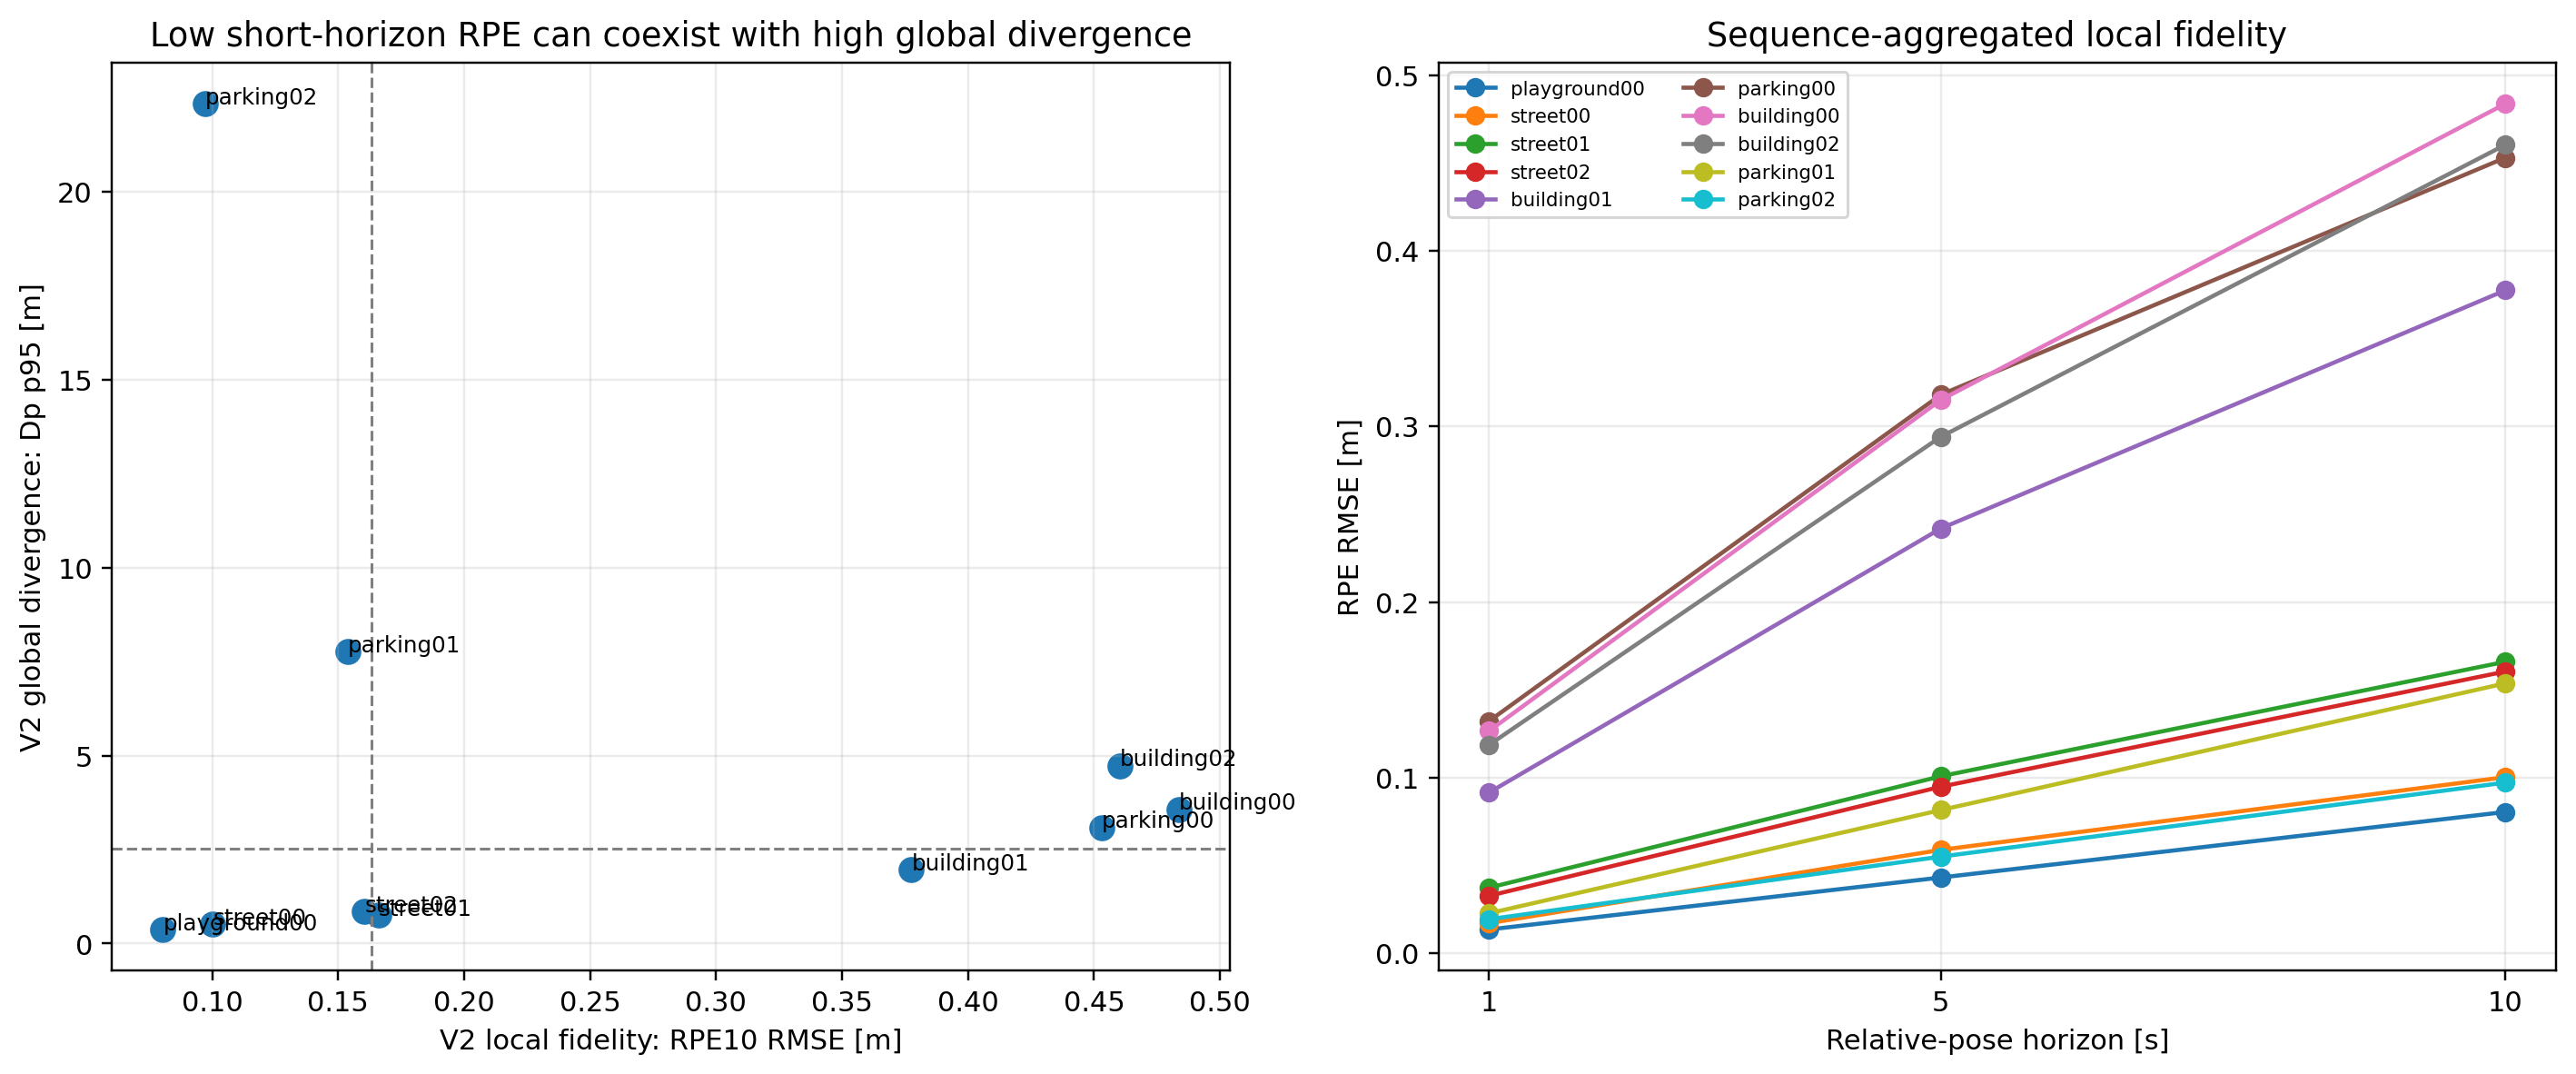
\includegraphics[width=\columnwidth]{local_vs_global_fidelity.png}
\caption{Local versus global fidelity for representative frozen V2 sequences. Low RPE$_{10}$ does not guarantee low accumulated physical--virtual divergence.}
\label{fig:localglobal}
\end{figure}

\subsection{Mechanism and Condition Dependence}
The strongest local/global contrast is observed in \texttt{parking02}: ATE $=11.350$~m, RPE$_{10}=0.097$~m, $Dp$ p95 $=22.345$~m, and $\Dtheta$ p95 $=30.415^{\circ}$. \texttt{parking01} provides a corroborating, less extreme case with ATE $=4.071$~m and RPE$_{10}=0.154$~m. Across the ten physical sequences, persistent signed yaw mismatch is strongly associated with accumulated yaw residual (Pearson $r=0.974$), and heading divergence is strongly associated with position divergence (Pearson $r=0.988$). The intermediate accumulated-yaw-to-heading relationship is weaker and non-monotonic (Pearson $r=0.381$), so the mechanism is a measured pathway rather than a universal causal law.

Condition analysis confirms that different contexts degrade different fidelity dimensions. High wheel--IMU disagreement increases RPE$_1$ in all ten sequences; high turning increases RPE$_5$ and RPE$_{10}$ in nine of ten; high acceleration increases $Dp$ p95 in nine; and high curvature increases $\Dtheta$ p95 in all ten. This supports a componentwise, condition-dependent profile instead of one scalar score.

\begin{figure}[t]
\centering
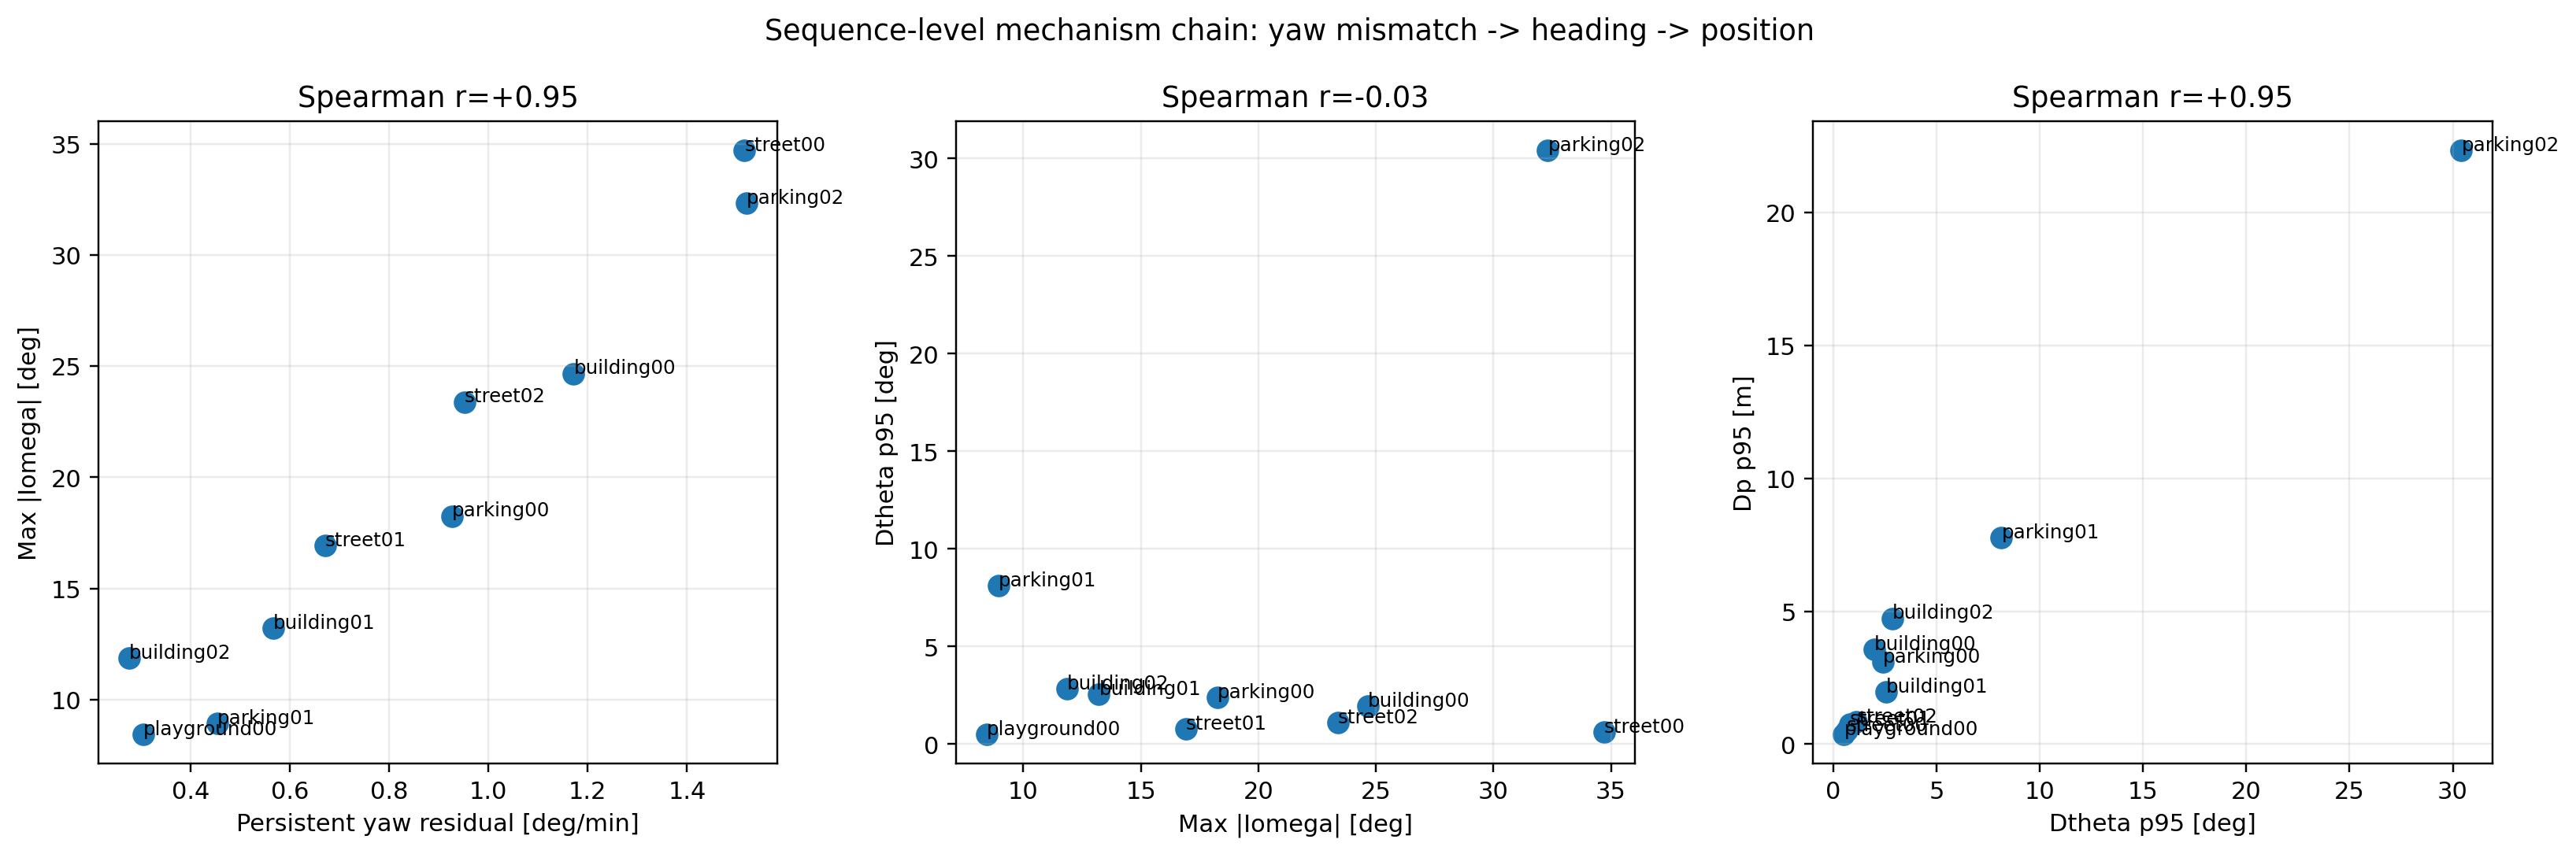
\includegraphics[width=\columnwidth]{persistent_yaw_mechanism.png}
\caption{Sequence-level mechanism analysis linking persistent yaw mismatch to accumulated and global divergence.}
\label{fig:yawmechanism}
\end{figure}

\begin{figure}[t]
\centering
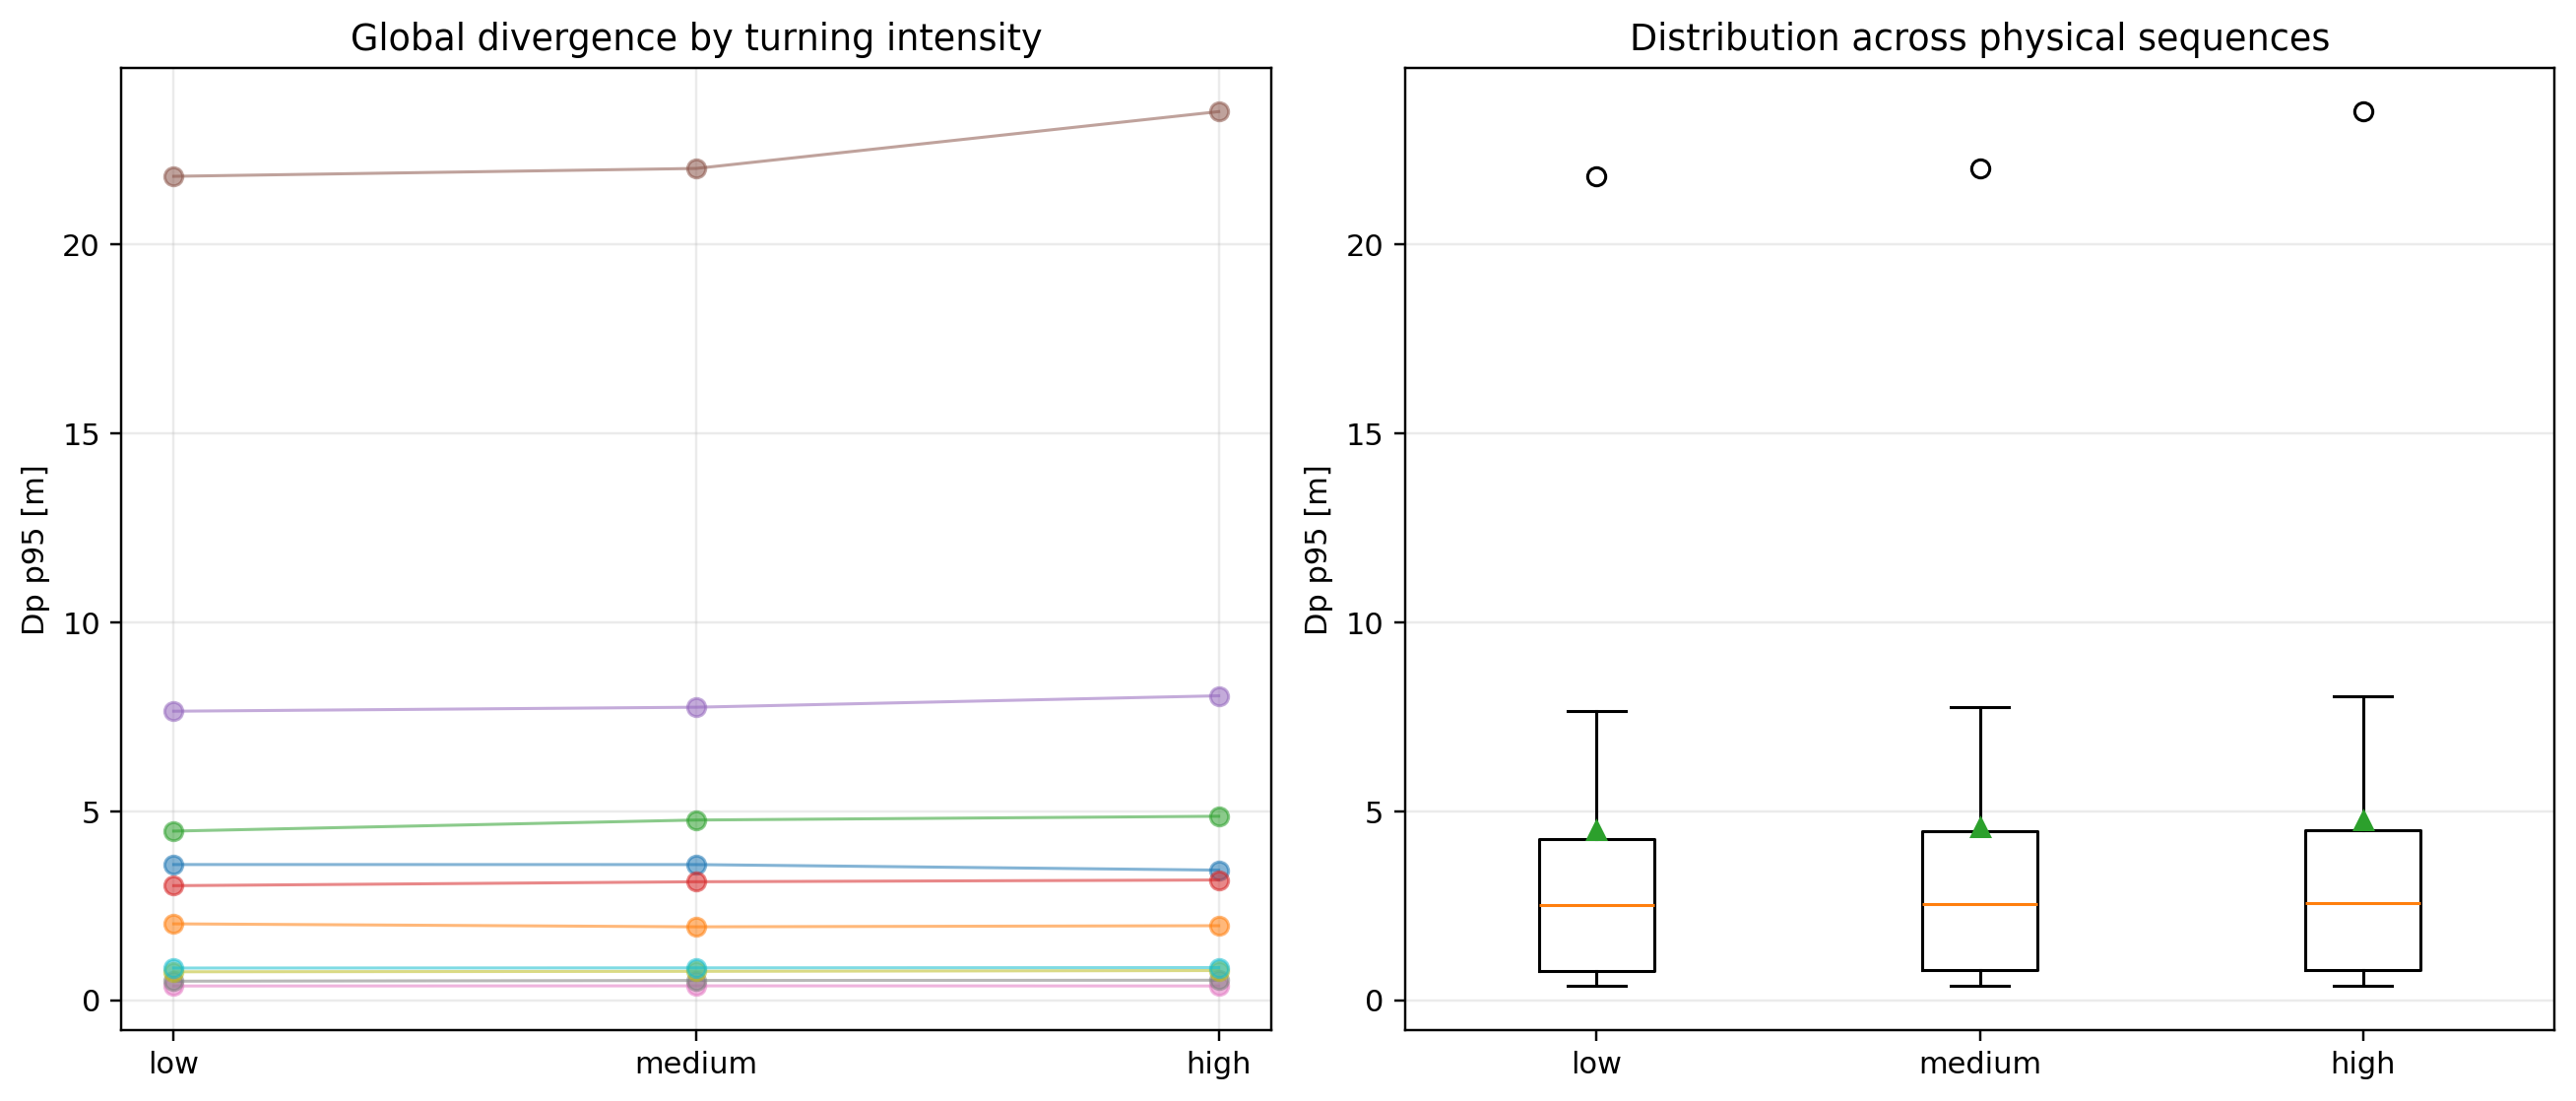
\includegraphics[width=\columnwidth]{condition_dependent_fidelity.png}
\caption{Condition-dependent fidelity: turning intensity is associated with degradation of finite-horizon relative motion.}
\label{fig:conditions}
\end{figure}

\subsection{Empirical Benign Fidelity Envelope}
For benign operation, the study estimates the componentwise distribution $\mathcal{P}_{\mathrm{benign}}(\mathbf{D}\mid c)$ using speed, acceleration, turning intensity, curvature, wheel--IMU disagreement, and elapsed-time regime. The envelope retains physical units and uses the 95th percentile descriptively; exceeding it is not interpreted as an attack, anomaly, failure, or untrustworthiness. The most important time dependence is that the $Dp$ p95 increases from 5.828~m in the early-run bin to 17.118~m in the late-run bin.

Leave-one-physical-sequence-out validation shows partial generalization. Mean held-out p95 coverage is 0.972 for $\Dv$, 0.975 for $\Domega$, 0.945 for $Dp$, and 0.915 for $\Dtheta$. Rate-domain quantities are therefore substantially more stable than global position and heading; \texttt{parking02} is the dominant difficult held-out case. Conditioning improves interpretation of where divergence occurs, but does not uniformly improve raw coverage because it often produces a tighter, more specific envelope.

\begin{figure}[t]
\centering
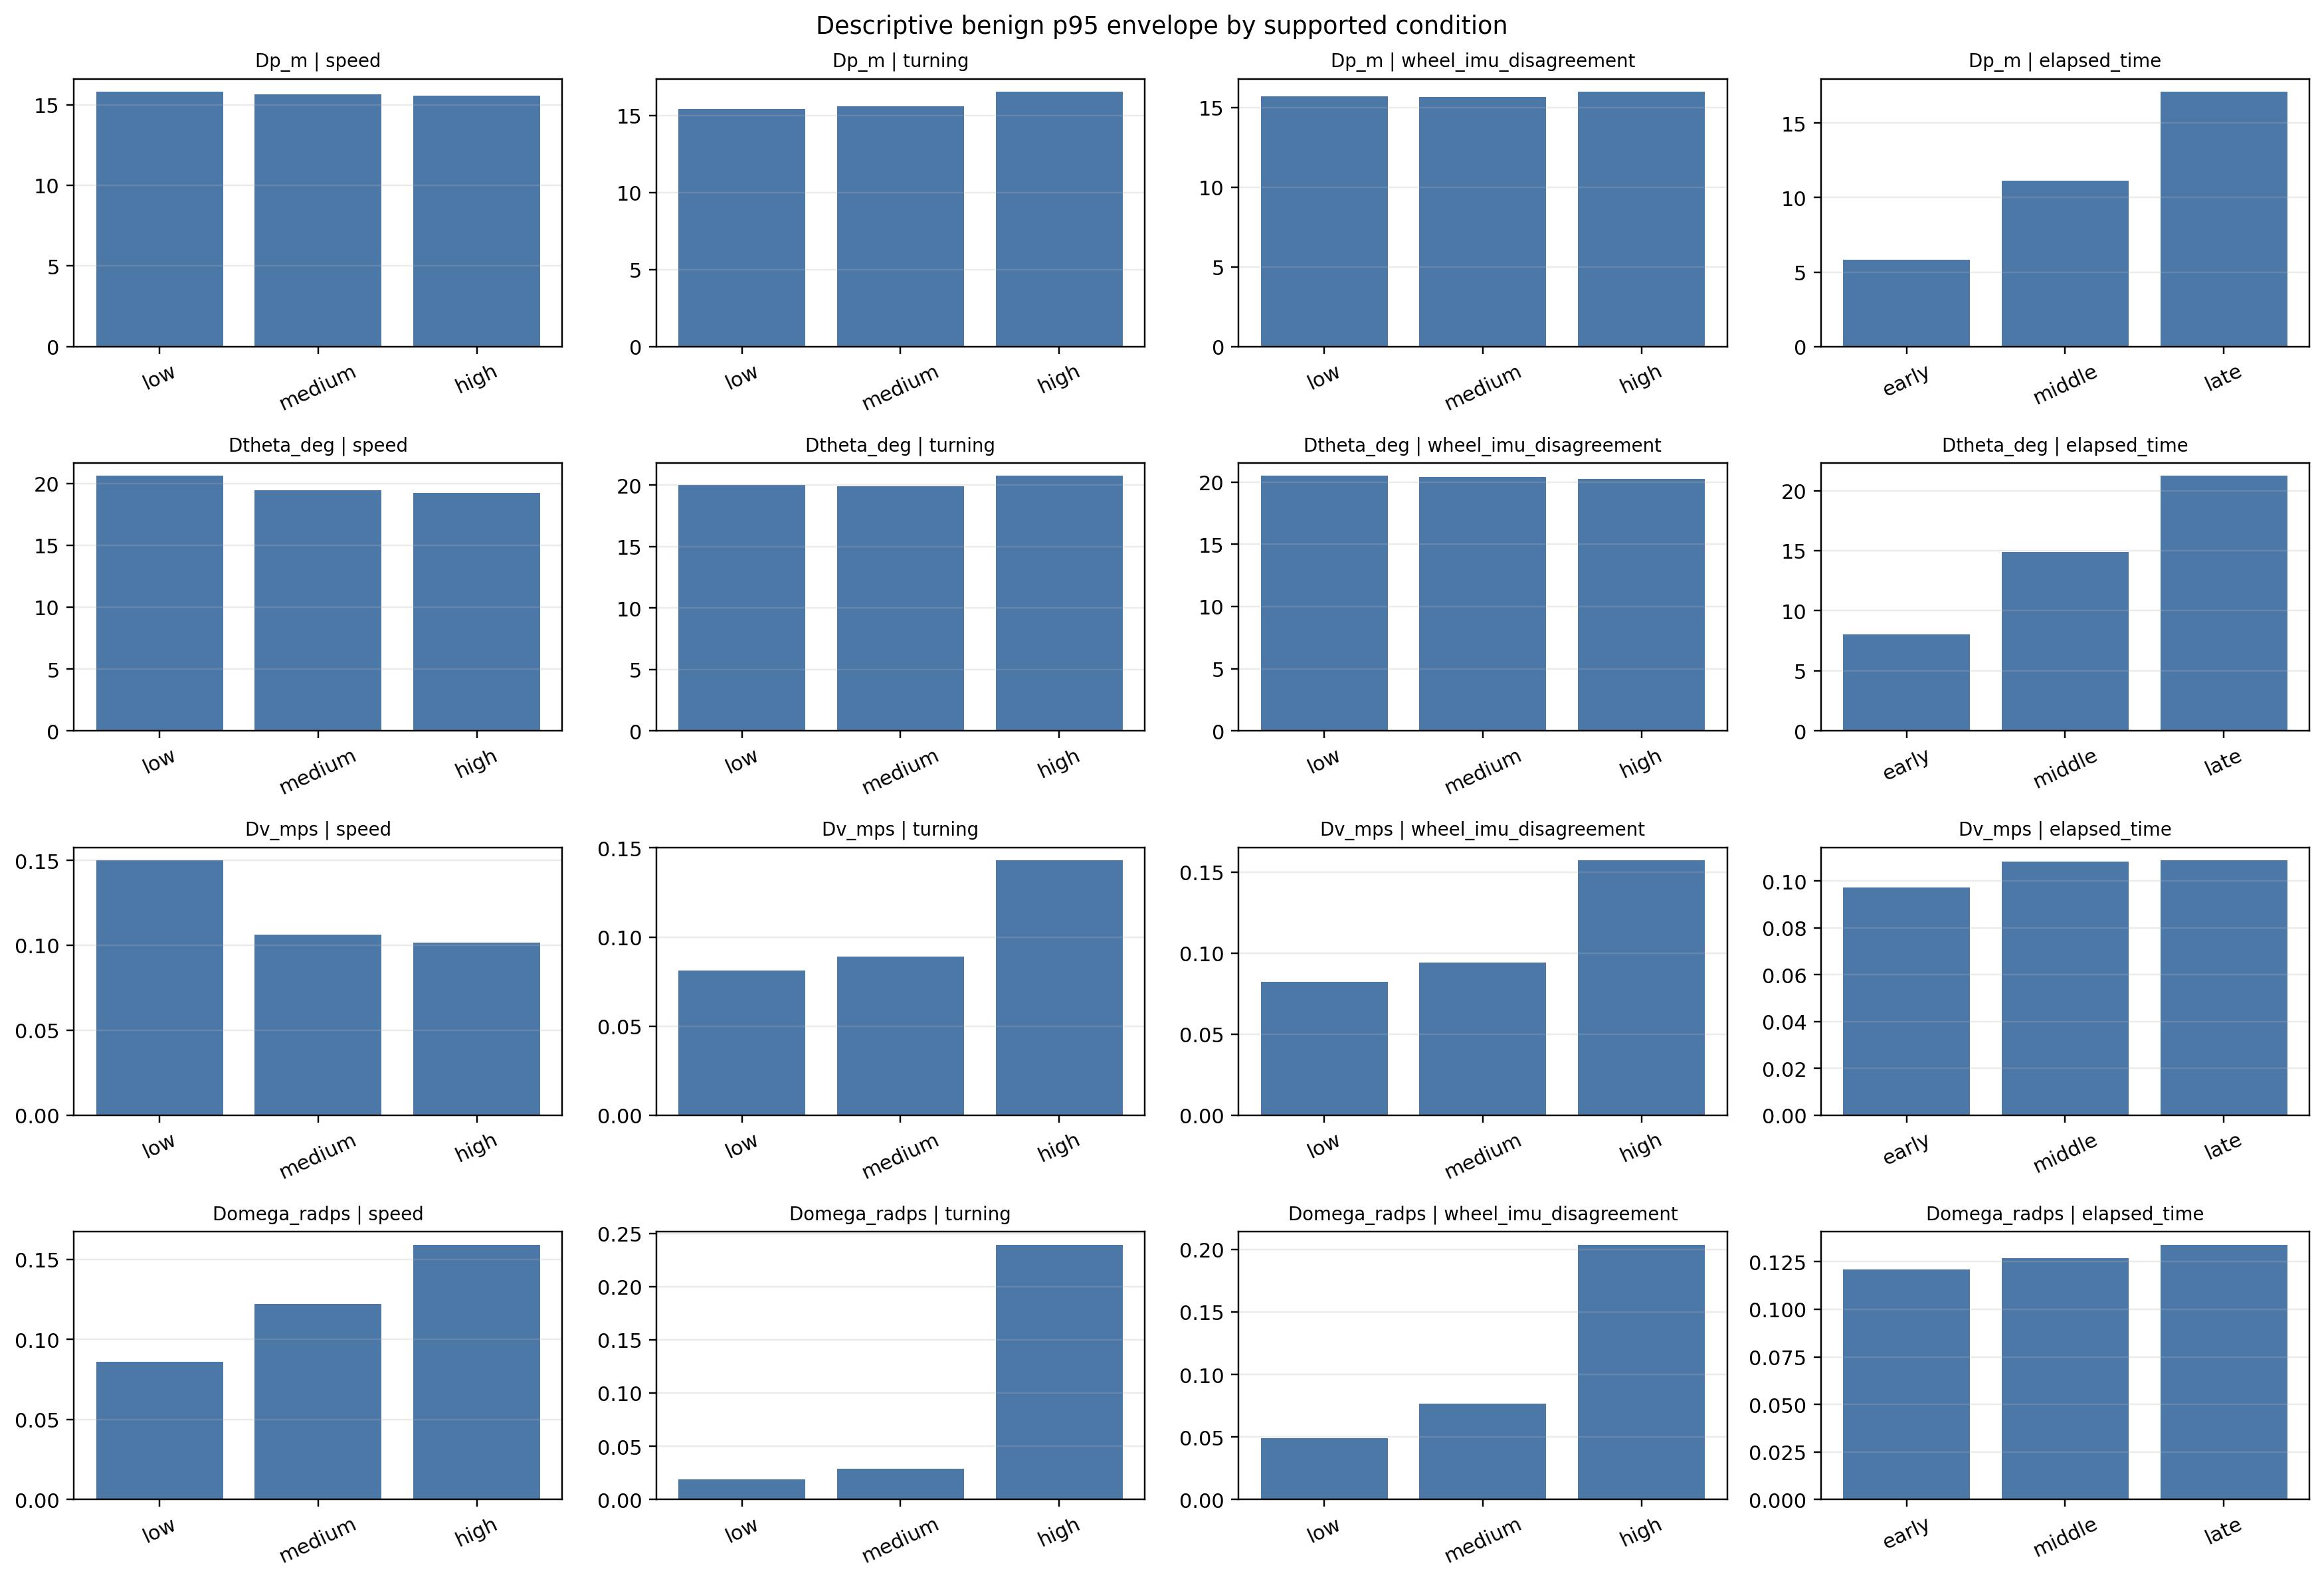
\includegraphics[width=\columnwidth]{benign_envelope_by_condition.png}
\caption{Componentwise empirical benign fidelity envelopes across operating contexts.}
\label{fig:envelope}
\end{figure}

\begin{figure}[t]
\centering
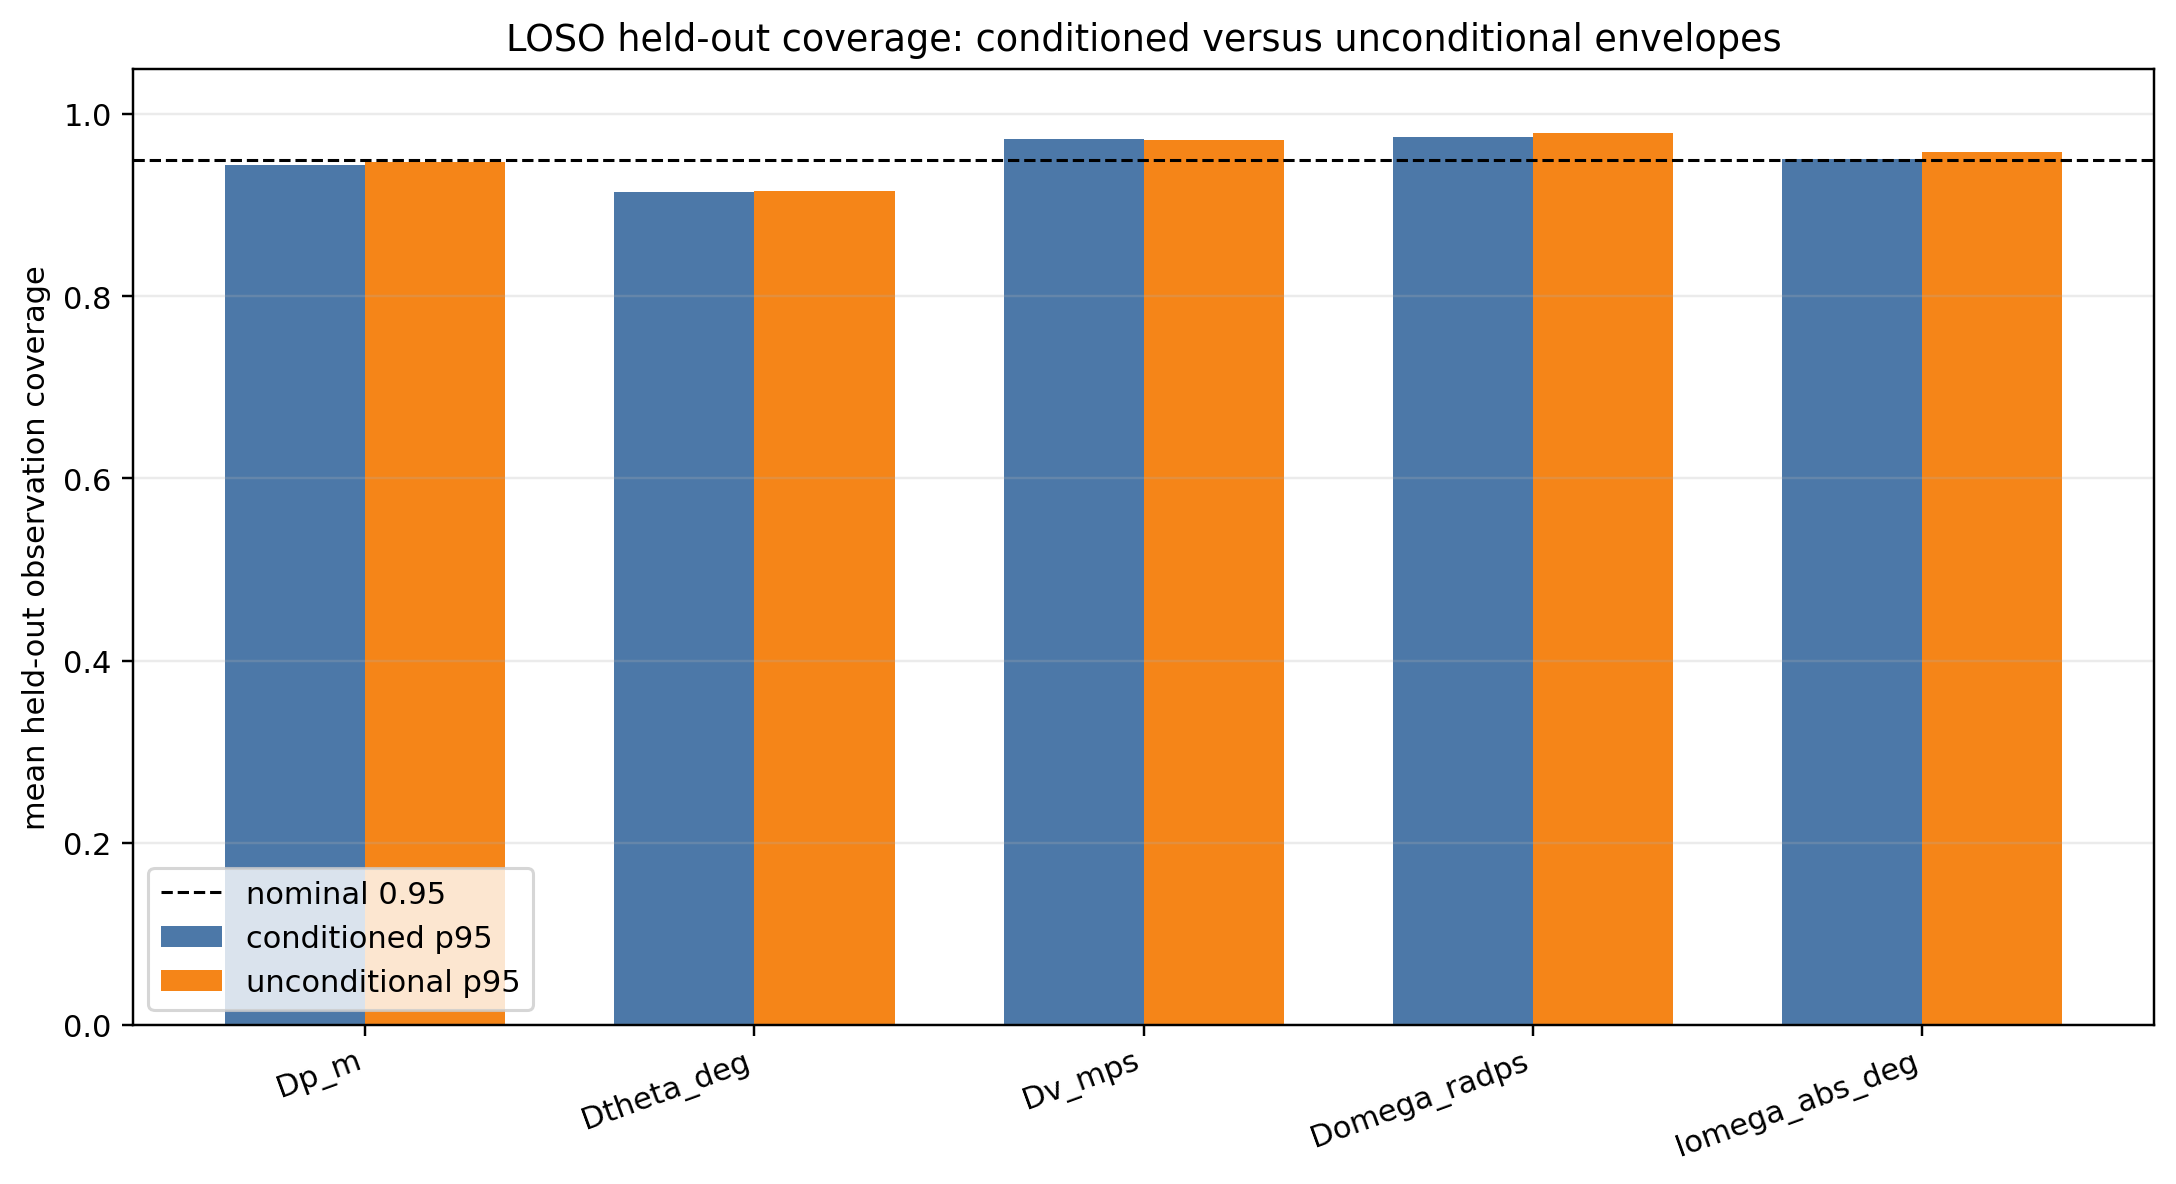
\includegraphics[width=\columnwidth]{loso_envelope_coverage.png}
\caption{Held-out benign-envelope coverage. Rate disagreement generalizes more reliably than global divergence.}
\label{fig:loso}
\end{figure}

\subsection{UGV01 Asset-Specific Instantiation}
The UGV01 study binds the representation to a tracked UGV01 using encoder conventions, AprilTag frame geometry, timing alignment, effective turning geometry, and low-speed carpet calibration. In the same-window comparison, ATE decreases from 0.131 to 0.099~m, RPE$_1$ from 0.035 to 0.028~m, and heading MAE from 13.3 to 5.6$^{\circ}$. The full repaired headline is ATE $=0.114$~m, RPE$_1=0.030$~m, RPE$_5=0.087$~m, RPE$_{10}=0.104$~m, and heading MAE $=6.7^{\circ}$. This is evidence of asset-specific improvement under the tested low-speed indoor carpet condition, not a universal all-surface claim.

\begin{figure}[t]
\centering
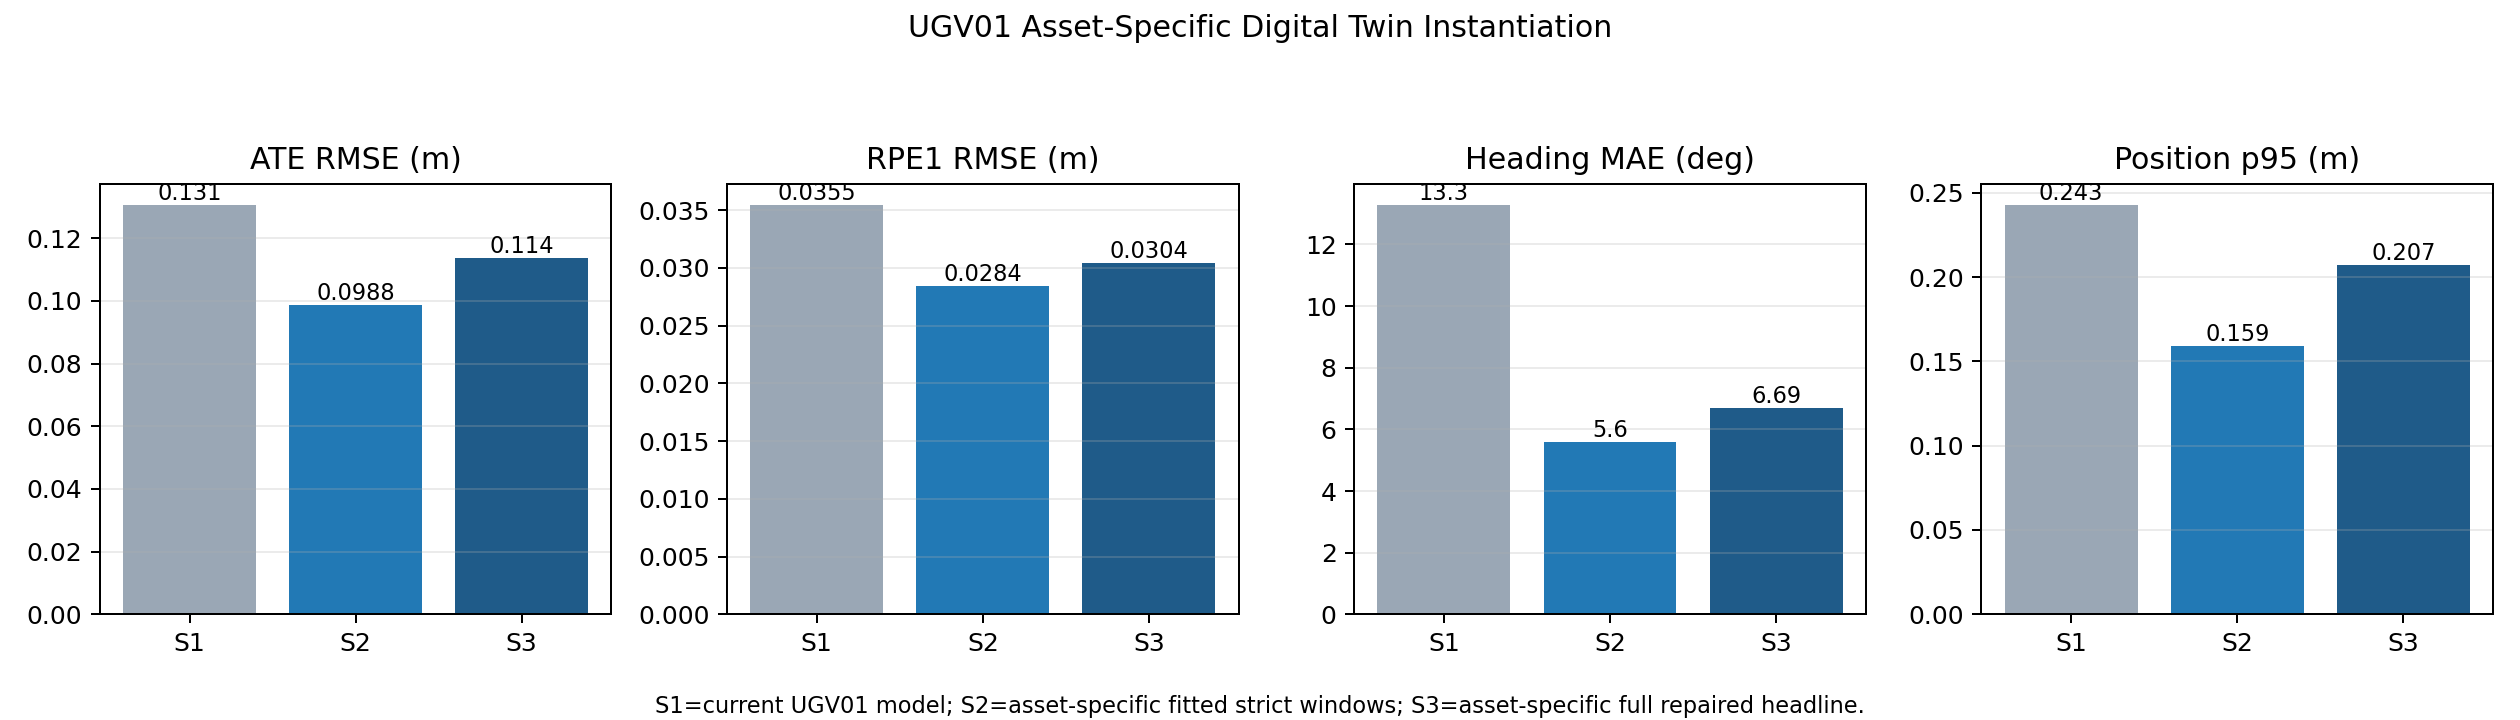
\includegraphics[width=\columnwidth]{ugv01_asset_instantiation.png}
\caption{UGV01 asset-specific calibration improves physical--virtual fidelity in the validated AprilTag-referenced condition.}
\label{fig:ugv01}
\end{figure}

To test whether the same local/global distinction appears on the physical rover, we applied the exact architecture-independent i2Nav fidelity evaluator to the accepted carpet run and two existing smooth-floor artifacts. The core metrics use the same 1, 5, and 10~s relative-motion definitions; the rate diagnostics are explicitly derived from finite differences of the aligned physical and twin poses because these UGV01 CSVs do not contain the original model prediction trace. Table~\ref{tab:ugv01conditions} shows that local RPE remains small across conditions, while heading and global divergence increase substantially on the smooth-floor square run. This is physical evidence for a condition-dependent fidelity profile and for the local-versus-global distinction, but the smooth-floor runs remain supplemental because their synchronization is motion-correlated and they are not repeated prospective trials.

\begin{table}[t]
\centering
\caption{UGV01 fidelity profile across existing AprilTag conditions using the exact i2Nav evaluator.}
\label{tab:ugv01conditions}
\footnotesize
\begin{tabular}{lrrrrrr}
\toprule
Condition & ATE & Head. & RPE$_1$ & RPE$_5$ & RPE$_{10}$ & $\Dp$ p95 \\
 & (m) & MAE ($^{\circ}$) & (m) & (m) & (m) & (m) \\
\midrule
Carpet, low speed & 0.114 & 6.7 & 0.029 & 0.086 & 0.109 & 0.207 \\
Smooth floor, trapezoid & 0.101 & 17.4 & 0.023 & 0.069 & 0.096 & 0.165 \\
Smooth floor, 1.5 m square & 0.338 & 28.6 & 0.021 & 0.057 & 0.089 & 0.918 \\
\bottomrule
\end{tabular}
\end{table}

\begin{figure}[t]
\centering
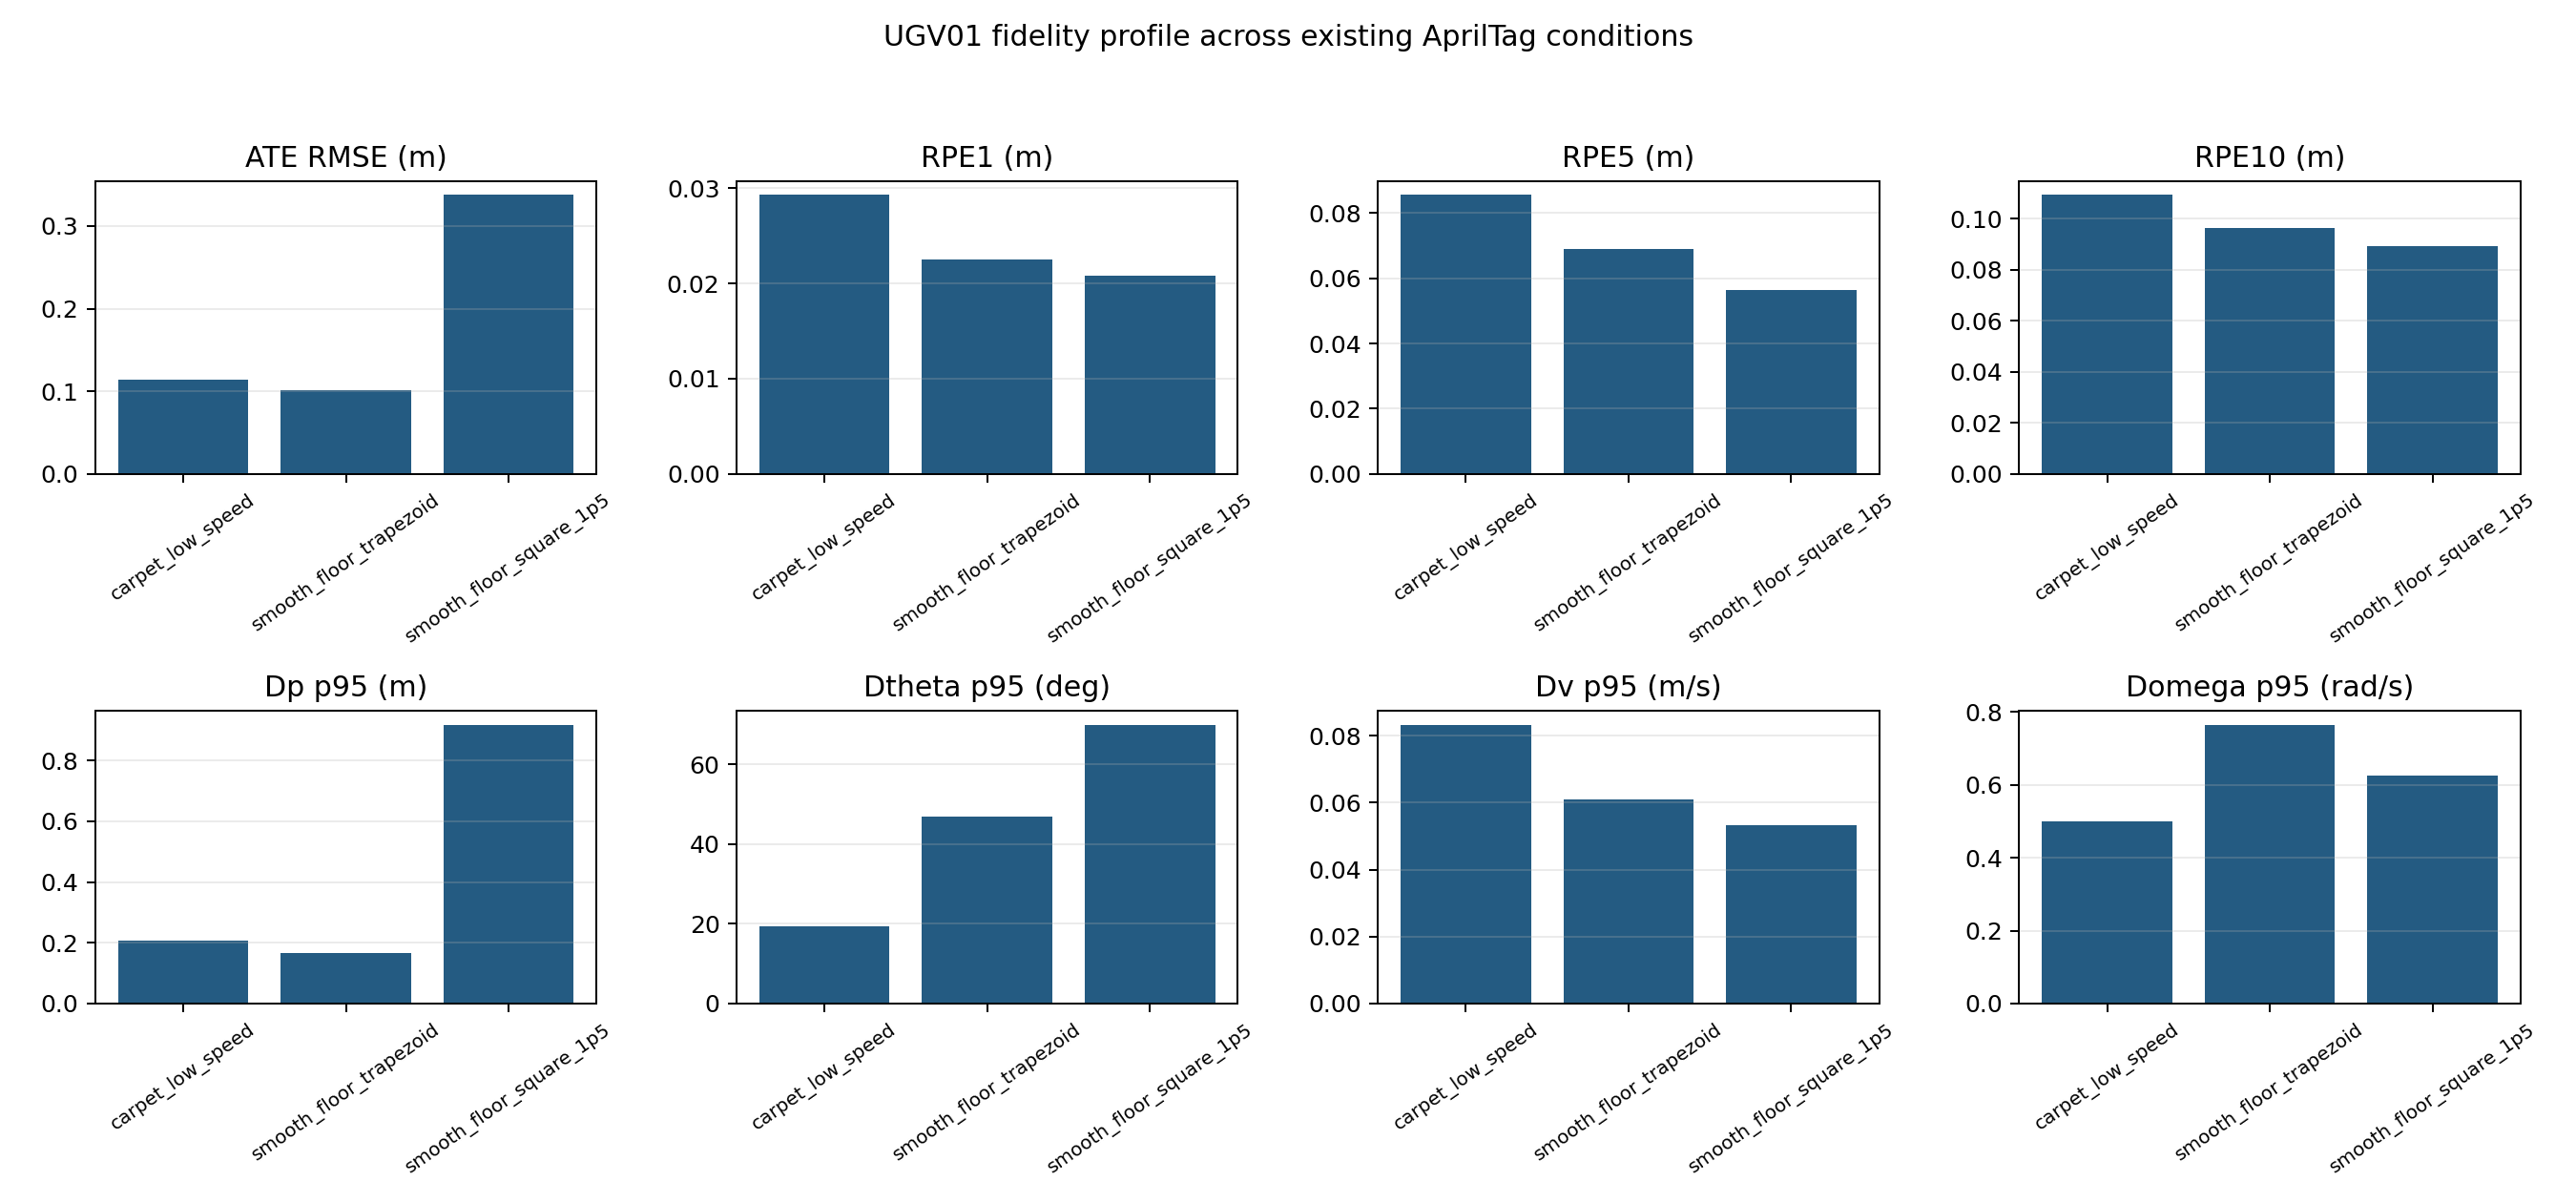
\includegraphics[width=\columnwidth]{ugv01_condition_fidelity_profile.png}
\caption{Dimension-by-dimension UGV01 fidelity across the existing carpet and smooth-floor AprilTag conditions.}
\label{fig:ugv01conditions}
\end{figure}

\begin{figure}[t]
\centering
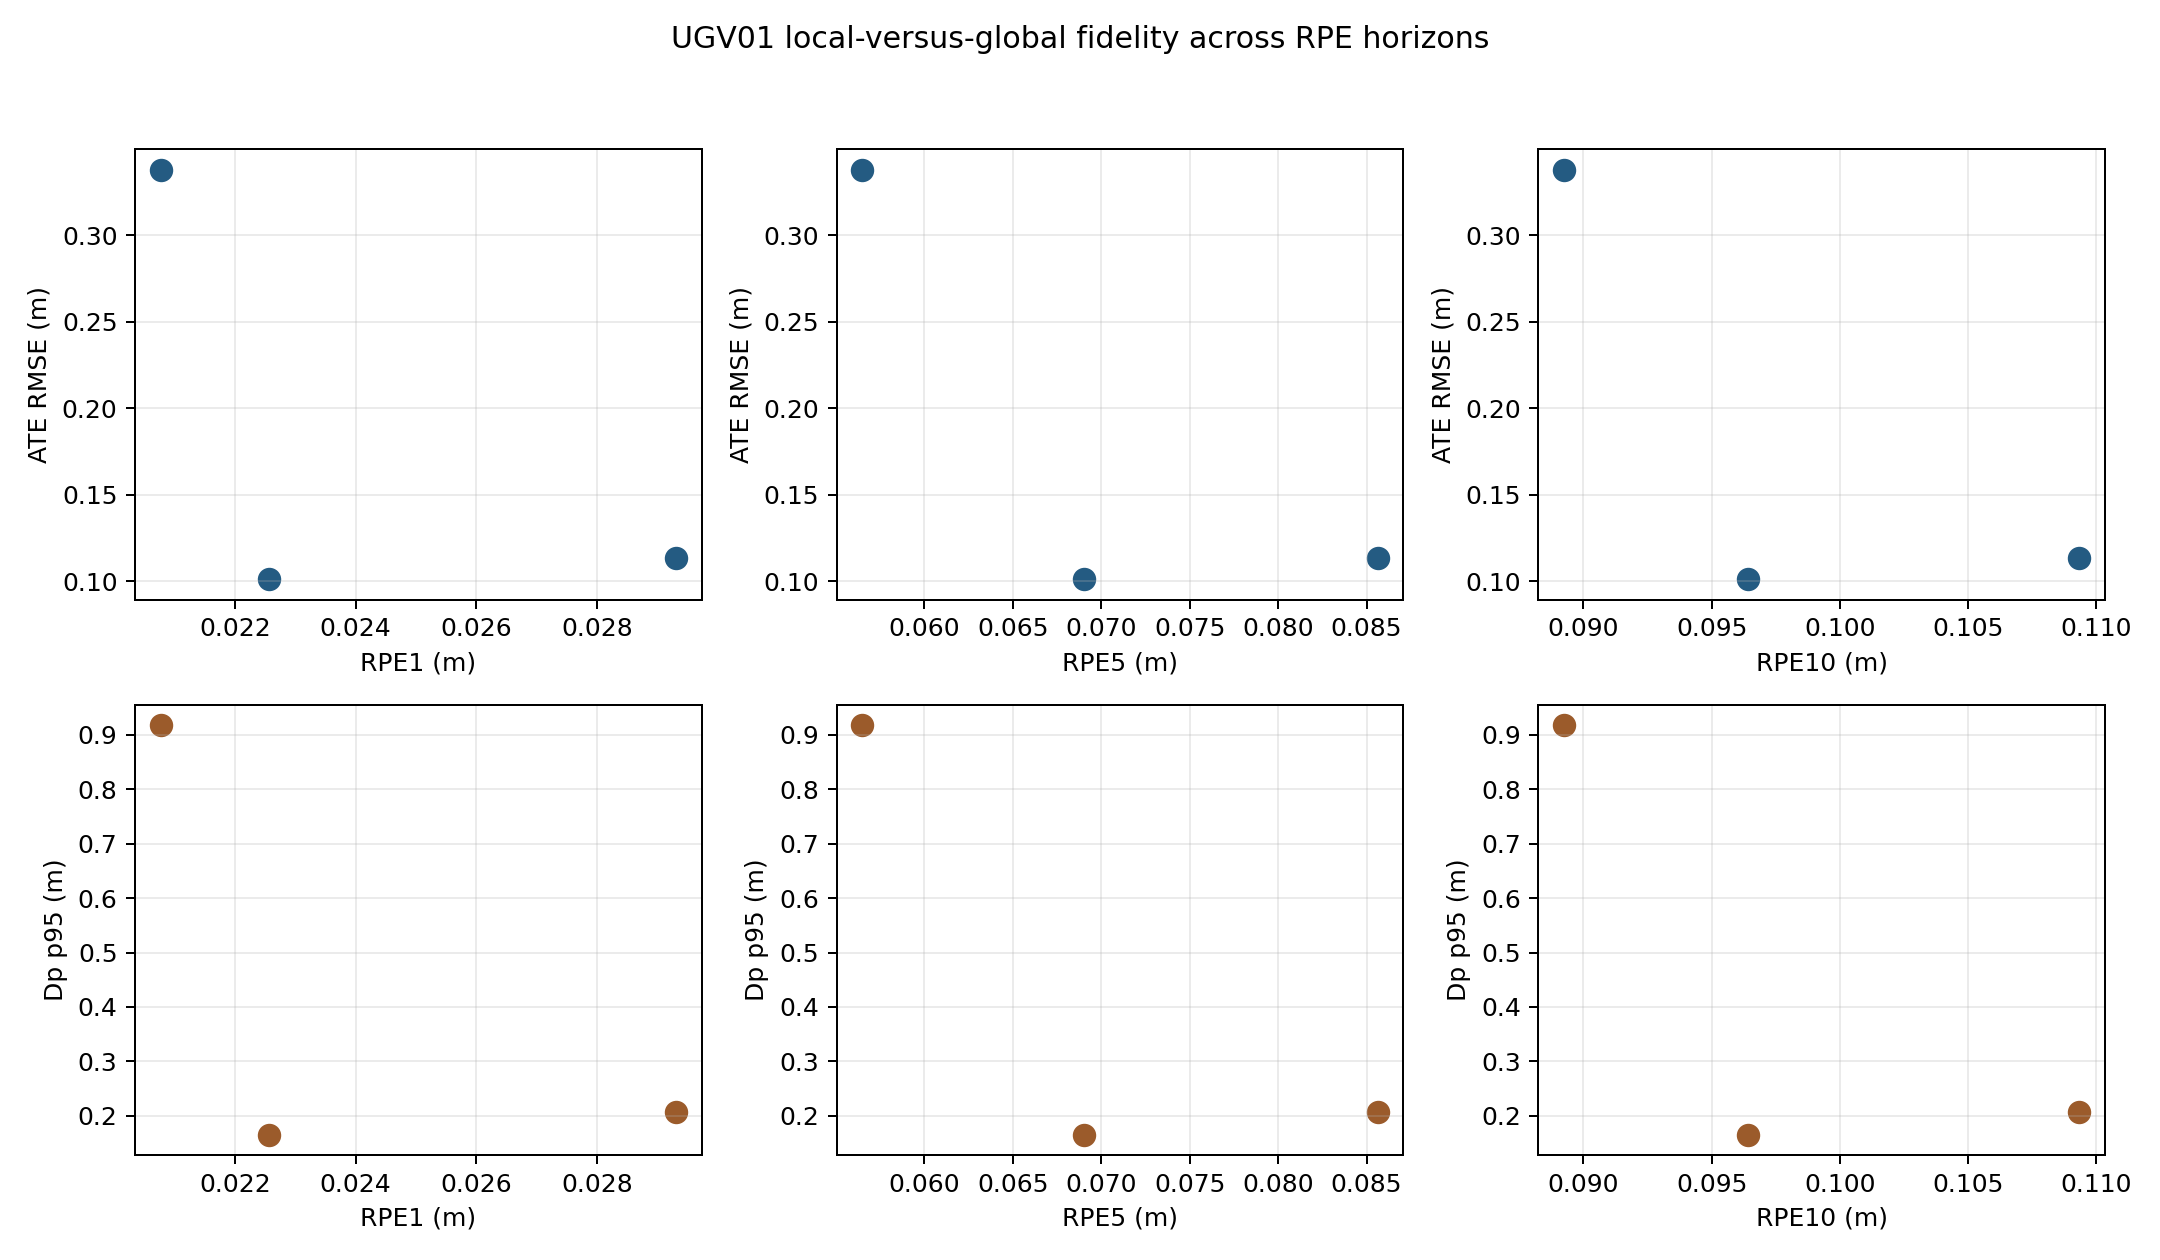
\includegraphics[width=\columnwidth]{ugv01_rpe_vs_global_fidelity.png}
\caption{UGV01 RPE$_1$/RPE$_5$/RPE$_{10}$ versus global ATE and $\Dp$ p95. Low local error can coexist with larger global divergence.}
\label{fig:ugv01localglobal}
\end{figure}

\subsection{Official Benchmark Positioning}
The official i2Nav benchmark is reported separately from operational DT fidelity because it applies standardized trajectory alignment. Twin V2 has official APE translation macro mean 1.635~m and rotation macro mean 3.011$^{\circ}$, with RPE translation values of 1.310~m at 50~m, 2.217~m at 100~m, and 3.635~m at 300~m. Relative to the available Fixed Physics comparator (3.299~m APE translation), this is a 50.4\% reduction in macro-mean APE; the separate mean sequence-wise relative reduction is 34.9\%. These quantities must not be conflated. An equivalent frozen V1 export was unavailable, so no official V1 comparison is claimed. In sensing context, V2 uses only wheel/odometry and IMU at runtime and ranks 5/9 among the directly comparable i2Nav ATE/ARE rows; it is not claimed to outperform heavier visual or LiDAR systems.

\begin{figure}[t]
\centering
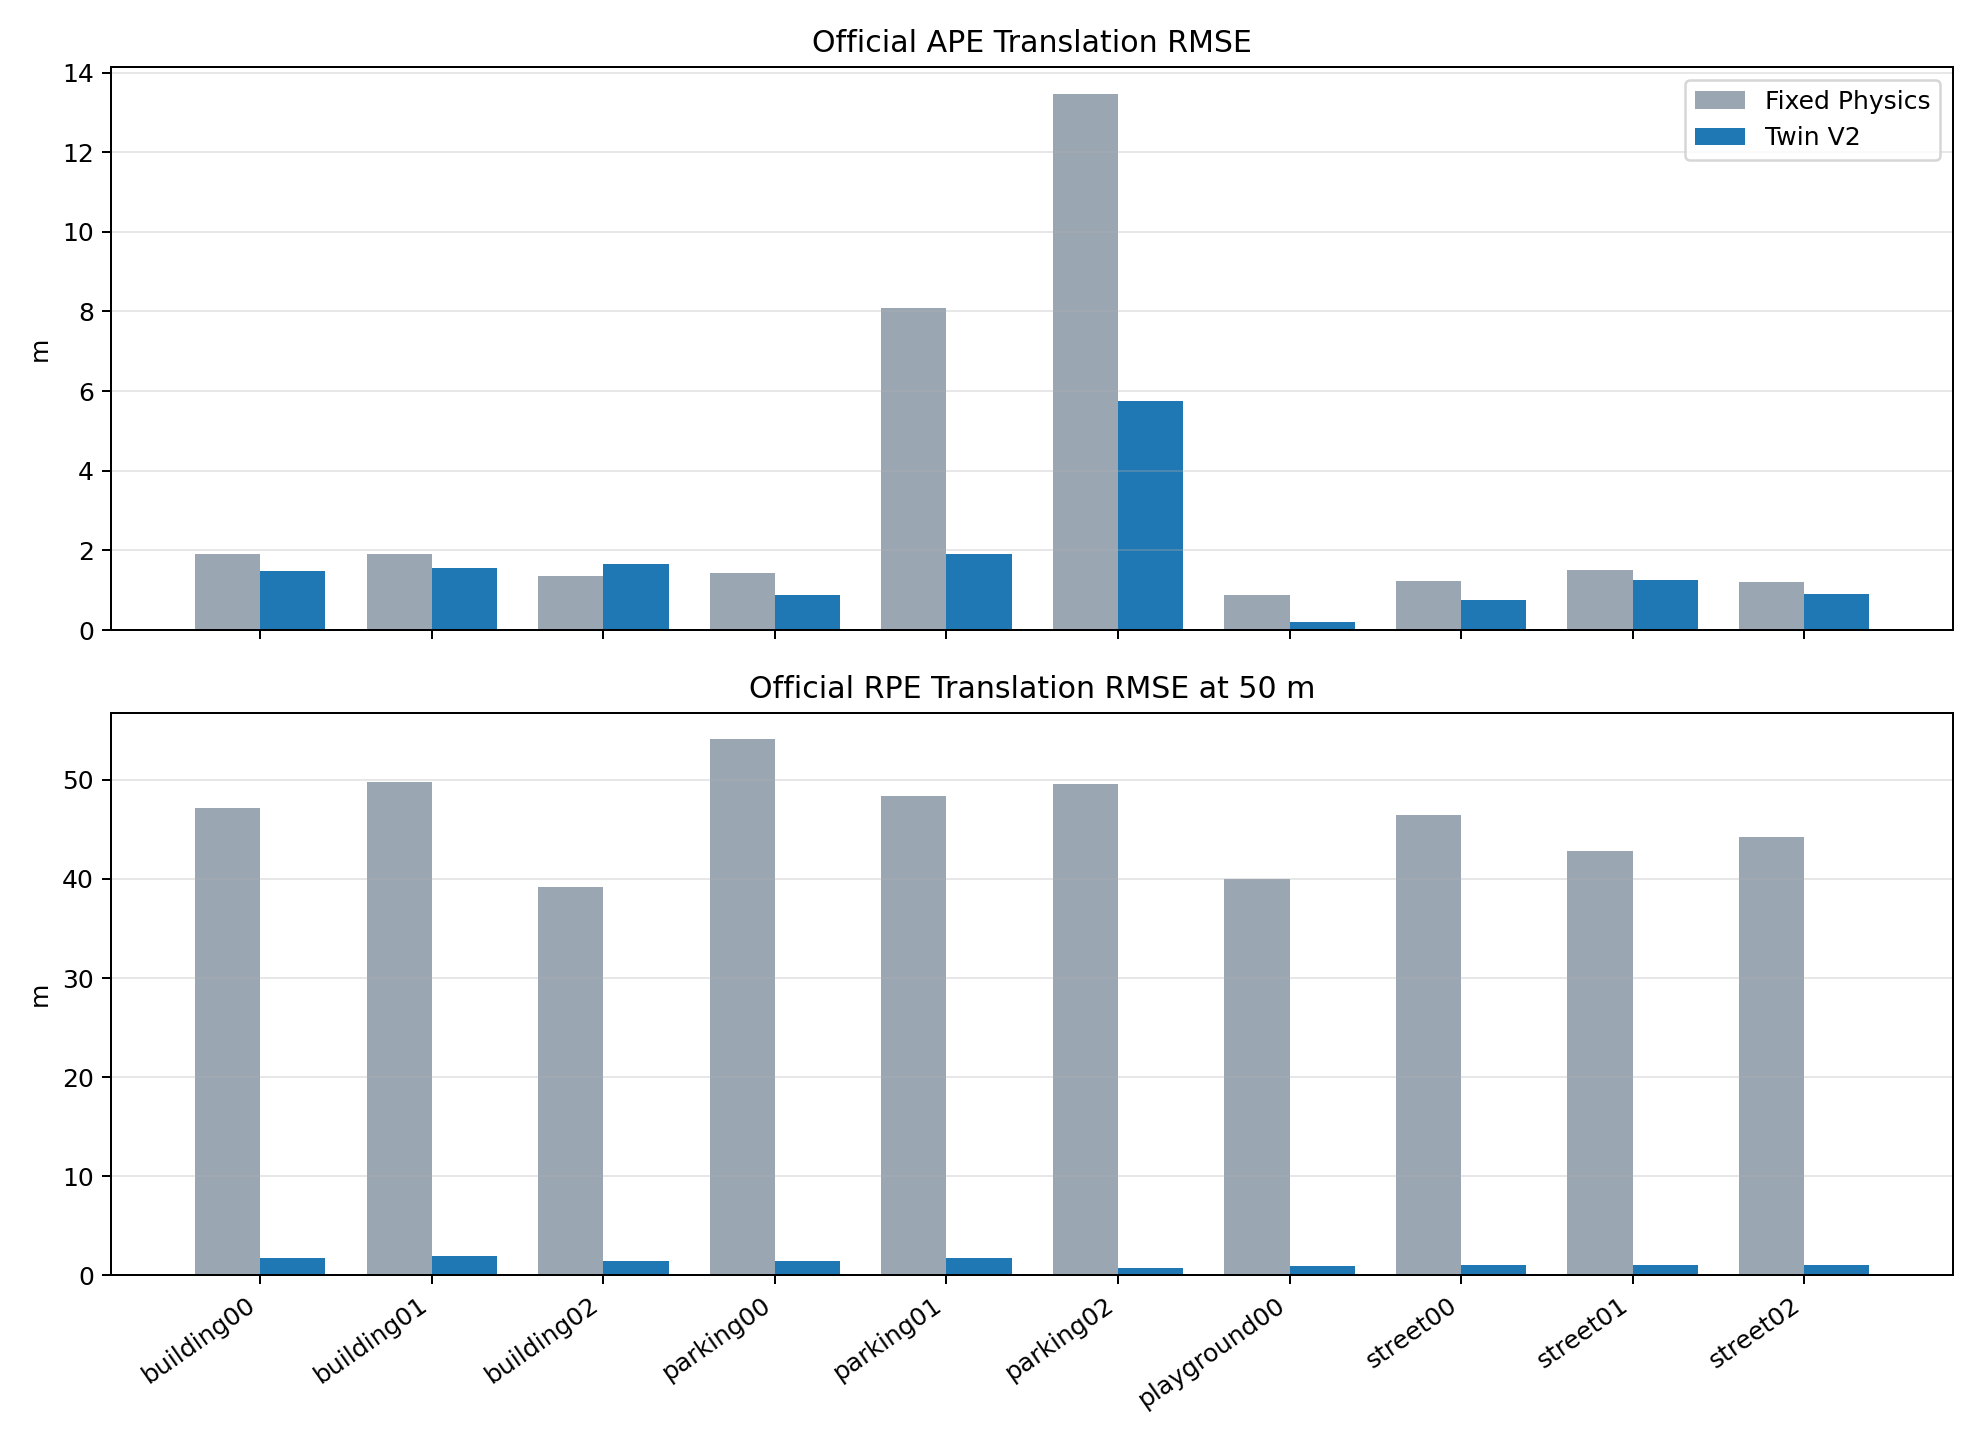
\includegraphics[width=\columnwidth]{official_benchmark_results.png}
\caption{Official i2Nav benchmark positioning, reported separately from the internal physical--virtual fidelity framework.}
\label{fig:official}
\end{figure}

\begin{figure}[t]
\centering
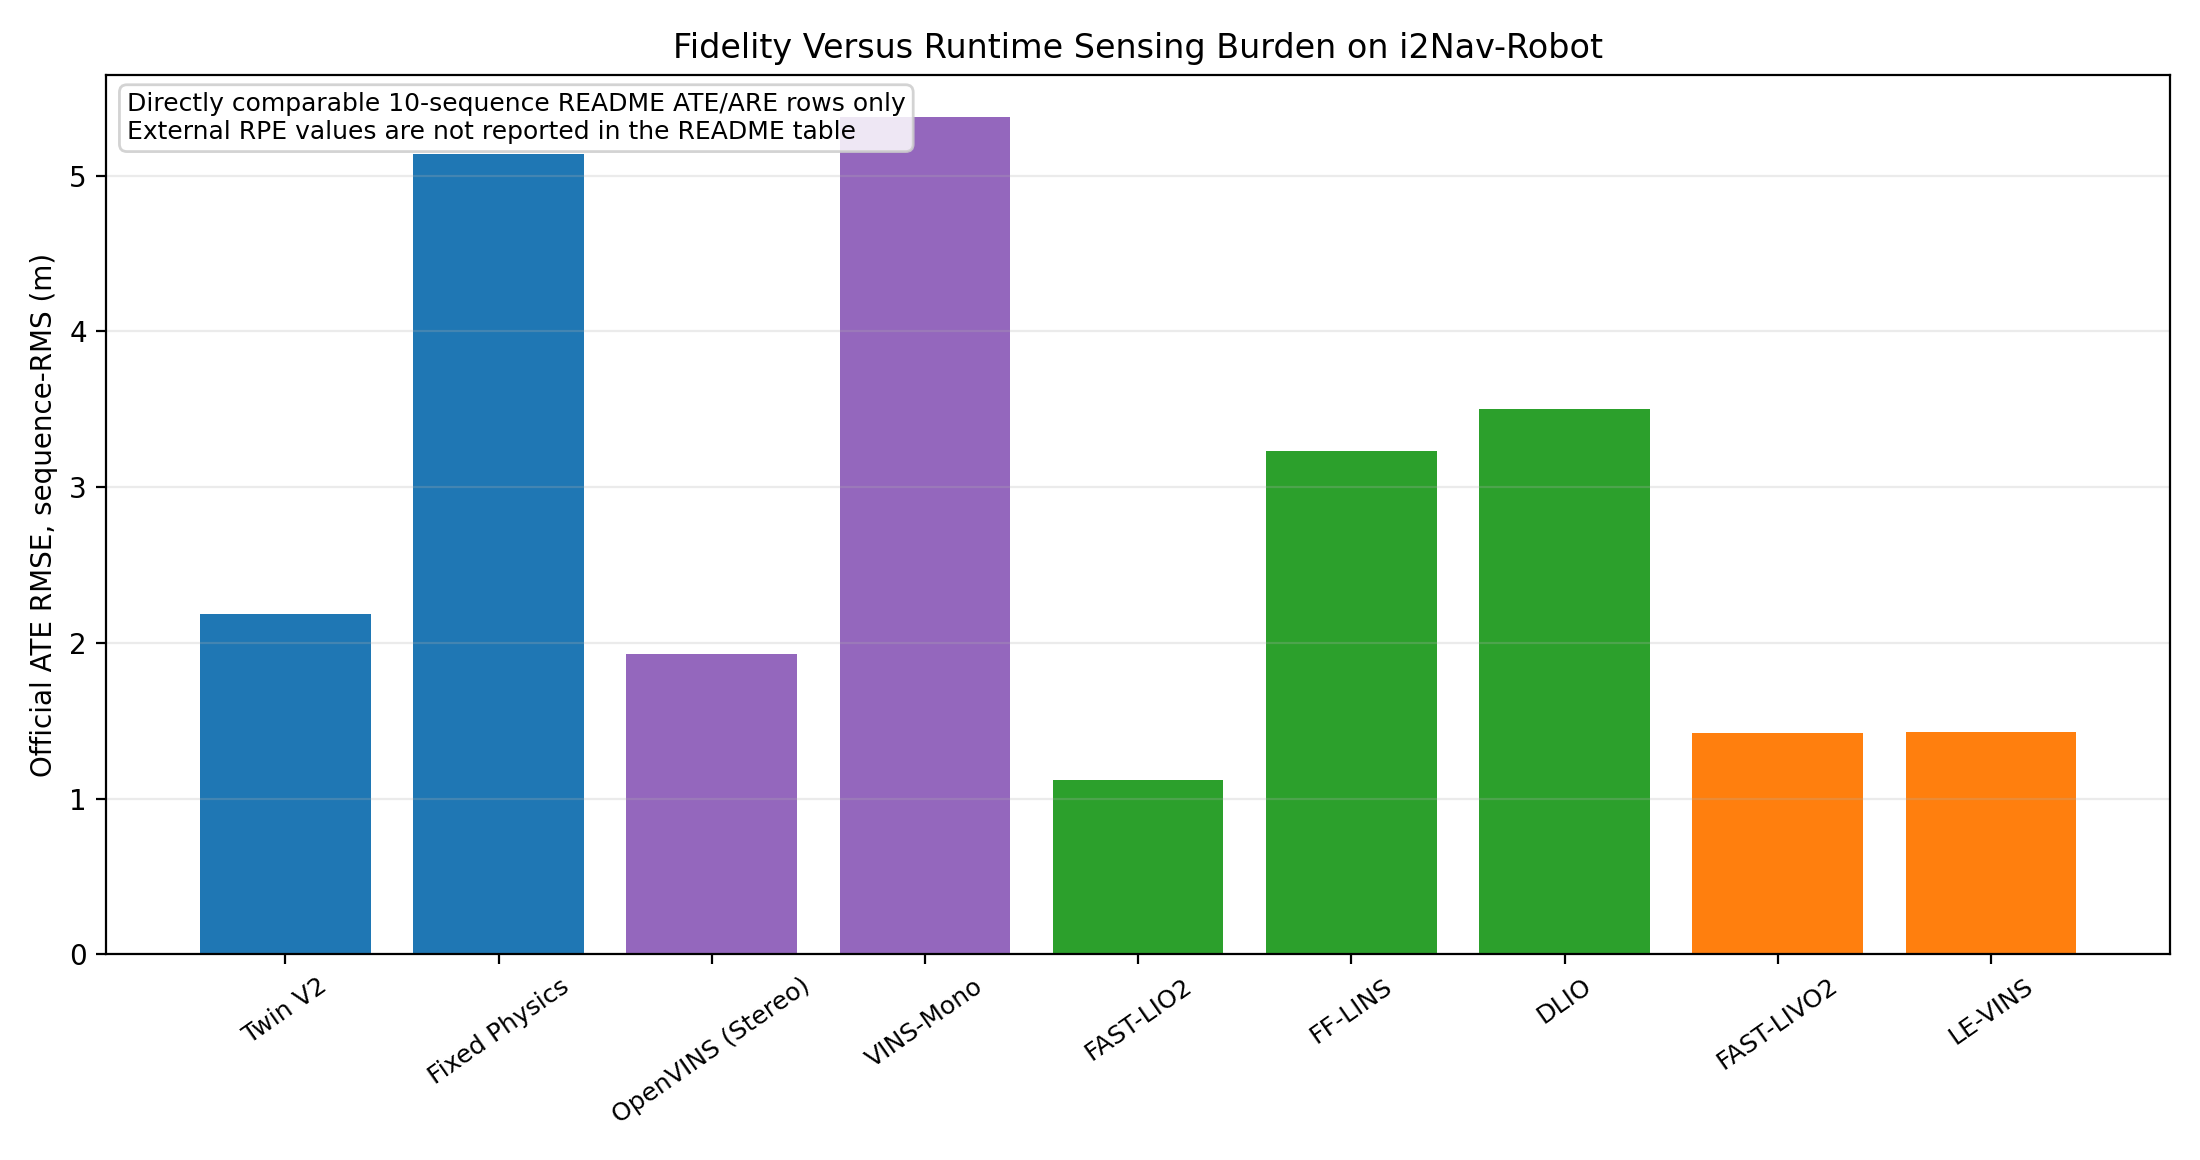
\includegraphics[width=\columnwidth]{sensing_fidelity_tradeoff.png}
\caption{Sensing--fidelity context on i2Nav. Twin V2 uses wheel/odometry and IMU only at runtime; heavier systems remain more accurate on this benchmark.}
\label{fig:sensing}
\end{figure}

\section{Research Status}
Table~\ref{tab:status} separates completed work from the evidence still required before publication-grade claims can be made.

\begin{table*}[t]
\centering
\caption{Research status as of August 2026.}
\label{tab:status}
\footnotesize
\begin{tabular}{p{0.7cm} p{4.0cm} p{2.0cm} p{8.0cm}}
\toprule
\textbf{Step} & \textbf{Task} & \textbf{Status} & \textbf{Current evidence / remaining requirement} \\
\midrule
0 & Freeze Twin V1 & Complete & Frozen baseline retained for paired comparison. \\
1 & Physical residual attribution & Substantially complete & Forward/yaw residuals, persistent bias, lateral/slip proxies, and sequence relationships computed. \\
2 & Diagnose \texttt{parking02} & Substantially complete & Persistent yaw mismatch is the dominant global-divergence mechanism; oracle yaw correction explains most fixed-model ATE. \\
3 & Formal DT fidelity/trust framework & Complete & Multidimensional divergence, finite-horizon/global metrics, residual diagnostics, statistical hierarchy, and empirical benign envelope are specified and evaluated. \\
4 & Residual-driven Twin V2 & Frozen & Slow persistent yaw correction plus fast mean-neutral transient correction; no learned yaw scale. \\
5 & Three-fold, three-seed pilot & Complete & Pilot informed V2 design and is superseded for aggregate claims by the frozen full-LOSO study. \\
6 & Full reproducibility evaluation & Complete & 10 held-out sequences $\times$ 3 seeds with sequence-level paired statistics and confidence intervals. \\
7 & Condition-dependent fidelity & Complete & Frozen bins evaluated for speed, acceleration, turning, curvature, wheel--IMU disagreement, and elapsed time. \\
8 & Official i2Nav evaluation & Complete with caveats & Protocol-audited official export and scoring; V1 equivalent export unavailable. \\
9 & Sensor--fidelity positioning & Complete with caveats & Runtime sensing inventory and protocol-compatible comparison; no Pareto/SOTA claim. \\
10 & Asset-specific instantiation study & Complete with scope limits & AprilTag-referenced UGV01 calibration comparison completed for low-speed indoor carpet. \\
11 & Cross-platform portability & Supporting evidence & i2Nav is the external benchmark; broader target-robot portability remains future work. \\
12 & Benign trust envelope & Complete descriptively & Componentwise envelope and LOSO validation completed; global dimensions remain sequence-sensitive and descriptive. \\
\bottomrule
\end{tabular}
\end{table*}

\section{Remaining Scope and Reproducibility Notes}
The core fidelity study is complete enough for manuscript submission. Remaining work is targeted validation and presentation, not another round of unconstrained architecture tuning.

\subsection{Frozen Evaluation Boundary}
Twin V2, its checkpoints, condition definitions, and evaluation protocol are frozen. All aggregate claims in this manuscript use the completed 10-sequence, three-seed LOSO outputs and the recorded provenance manifest.

\subsection{Reproducibility and Physical Validation}
The architecture-independent evaluator and full result archive are available. The most valuable remaining physical experiment is an untouched synchronized UGV01 repeat, ideally on a second surface or at a higher-motion condition, to test whether the AprilTag-referenced asset-specific result generalizes beyond the current low-speed carpet window.

\subsection{Interpretation Boundary}
Official aligned benchmark numbers and internal operational synchronization numbers remain in separate tables. The official result is useful for protocol-compatible positioning, while the internal profile is the evidence for the paper's DT-fidelity thesis.

\subsection{Optional Targeted UGV01 Extension}
The current paper can report the existing UGV01 result with its condition-limited scope. A second surface, higher speed, sustained turning, or controlled slip would each support one additional generalization claim; none is required to describe the completed existing-data analysis.

\subsection{Asset-Specific Claim Boundary}
The UGV01 instantiation result supports a claim for the tested low-speed indoor carpet condition. It does not establish all-surface, high-speed, or slip-heavy fidelity. Those claims should be added only after targeted physical validation.

\subsection{Official Benchmark and Sensing Position}
The official i2Nav export and scoring are complete. The appropriate conclusion is a sensor-lightweight positioning statement: V2 uses wheel/odometry and IMU at runtime, but heavier visual/LiDAR systems remain more accurate on the official trajectory metrics.

\subsection{Cross-Platform Template Portability}
The frozen source twin will be evaluated on external platforms. Zero-shot testing should be described as portability of the generic twin template, not automatically as a fully instantiated DT of the target robot. Limited target-robot calibration can then be evaluated as the process of re-instantiating that template for a new physical asset. No target-domain tuning is allowed for a strict zero-shot claim.

\subsection{Benign Trust Boundary}
The componentwise benign envelope and leave-one-sequence-out validation are complete. The envelope is a descriptive characterization of benign disagreement, not a universal alarm threshold; global position and heading remain sequence-sensitive.

\section{How This Work Strengthens the Security Study}
The security value of a DT depends on whether the virtual counterpart is sufficiently faithful to the physical asset. If benign sensor bias, slip, or model mismatch can already generate large divergence, a detector that alarms on physical--virtual disagreement may confuse normal modeling error with malicious manipulation. The present fidelity study therefore provides the missing baseline for the subsequent cyber-security paper.

Conceptually, the two-paper sequence is
\begin{equation}
\text{physical asset}
\rightarrow \text{validated twin}
\rightarrow \mathcal{P}_{\mathrm{benign}}(\mathbf{D}\mid c)
\rightarrow \text{attack/fault discrimination}.
\end{equation}
The later security paper can formulate
\begin{align}
H_0 &: \mathbf{D} \sim \mathcal{P}_{\mathrm{benign}}(\mathbf{D}\mid c),\\
H_1 &: \mathbf{D} \sim \mathcal{P}_{\mathrm{attack}}(\mathbf{D}\mid c),
\end{align}
with false-alarm rates grounded in measured benign twin behavior rather than arbitrary divergence thresholds. This also enables analysis of stealthy attacks that attempt to remain inside the normal fidelity envelope and clarifies which sensor/model residuals constitute trusted evidence.

\section{Current Claims and Explicit Non-Claims}
At the present research stage, the evidence supports the following statements:
\begin{itemize}
    \item A sensor-lightweight physical/learned replica can achieve strong finite-horizon fidelity on the current i2Nav experiments.
    \item Small persistent yaw mismatch can dominate long-horizon DT divergence while short-horizon RPE remains small.
    \item Frozen full-LOSO evaluation shows improved heading and longer-horizon fidelity, with short-horizon RPE preserved.
    \item Physical--virtual fidelity varies substantially by sequence/operating regime, motivating condition-dependent trust envelopes.
\end{itemize}

The evidence does \emph{not yet} support the following stronger claims:
\begin{itemize}
    \item that Twin V2 is globally superior across all ten i2Nav sequences or to heavier sensing systems;
    \item that \texttt{parking02} has reached high global fidelity;
    \item that a universal p95 threshold is a valid attack detector;
    \item that the generic zero-shot model is automatically a DT of a new physical robot;
    \item that the lightweight twin matches state-of-the-art heavier systems under the official i2Nav protocol;
    \item that the UGV01 result generalizes beyond the tested low-speed indoor carpet condition.
\end{itemize}
These claims are deliberately excluded unless the corresponding additional experiments are completed.

\section{Conclusion}
This paper frames the digital twin itself as the object of study. The completed evidence shows that a sensor-lightweight twin can provide useful short-horizon fidelity while still accumulating substantial long-horizon divergence, and that this distinction is explained in part by persistent yaw mismatch and operating conditions. The frozen full-LOSO evaluation, condition-dependent analysis, held-out benign-envelope validation, official i2Nav positioning, and UGV01 AprilTag instantiation together support a coherent methodology for measuring and diagnosing physical--virtual fidelity. The strongest remaining scientific limitation is external physical generalization: the UGV01 result is currently scoped to a low-speed indoor carpet condition. Subject to that limitation, the manuscript is ready to move from project-status framing into a conventional research-paper presentation, with the optional targeted UGV01 repeat identified as the next highest-value experiment.

\begin{thebibliography}{99}

\bibitem{dtc_definition}
Digital Twin Consortium, ``Definition of a Digital Twin,'' Digital Twin Consortium, accessed Aug. 17, 2026.

\bibitem{jones2020dt}
D. Jones, C. Snider, A. Nassehi, J. Yon, and B. Hicks, ``Characterising the Digital Twin: A systematic literature review,'' \emph{CIRP Journal of Manufacturing Science and Technology}, vol. 29, pp. 36--52, 2020, doi: 10.1016/j.cirpj.2020.02.002.

\bibitem{kober2023fidelity}
C. Kober, M. Fette, and J. P. Wulfsberg, ``A Method for Calculating Optimum Digital Twin Fidelity,'' \emph{Procedia CIRP}, vol. 120, pp. 1155--1160, 2023, doi: 10.1016/j.procir.2023.09.141.

\bibitem{zhang2025fidelity}
Y. Zhang, H. Sun, X. Zhang, and W. Liu, ``A fidelity evaluation method for digital twin model of aero-engine assembly characteristics,'' \emph{Journal of Manufacturing Systems}, vol. 78, pp. 444--456, 2025, doi: 10.1016/j.jmsy.2024.12.012.

\bibitem{ding2021robopheus}
X. Ding, H. Wang, H. Li, H. Jiang, and J. He, ``Robopheus: A Virtual-Physical Interactive Mobile Robotic Testbed,'' arXiv:2103.04391, 2021.

\bibitem{yang2025omr}
H. Yang, Z. Qin, Y. Xia, and F. Cheng, ``Digital Twin-Based Autonomous Navigation and Control of Omnidirectional Mobile Robots,'' \emph{IEEE Transactions on Vehicular Technology}, vol. 74, no. 4, pp. 5687--5697, 2025, doi: 10.1109/TVT.2024.3520991.

\bibitem{betzer2024runtime}
J. S. Betzer, J. Boudjadar, M. Frasheri, and P. Talasila, ``Digital Twin Enabled Runtime Verification for Autonomous Mobile Robots under Uncertainty,'' in \emph{Proc. 28th IEEE Int. Symp. Distributed Simulation and Real Time Applications (DS-RT)}, 2024, pp. 10--17, doi: 10.1109/DS-RT62209.2024.00012.

\bibitem{jiang2025wing}
C. Jiang, K. Zhang, S. Yang, S. Shen, C. Xu, and F. Gao, ``WING: Wheel-Inertial Neural Odometry with Ground Manifold Constraints,'' \emph{IEEE Transactions on Intelligent Vehicles}, vol. 10, no. 3, pp. 1510--1525, 2025, doi: 10.1109/TIV.2024.3429167.

\bibitem{tang2025i2nav}
H. Tang \emph{et al.}, ``i2Nav-Robot: A Large-Scale Indoor-Outdoor Robot Dataset for Multi-Sensor Fusion Navigation and Mapping,'' arXiv:2508.11485, 2025, doi: 10.48550/arXiv.2508.11485.

\bibitem{ma2024cps}
J. Ma, Y. Guo, C. Fang, and Q. Zhang, ``Digital-Twin-Based CPS Anomaly Diagnosis and Security Defense Countermeasure Recommendation,'' \emph{IEEE Internet of Things Journal}, vol. 11, no. 10, pp. 18726--18738, 2024, doi: 10.1109/JIOT.2024.3366904.

\bibitem{alcaraz2024anomaly}
C. Alcaraz and J. Lopez, ``Digital Twin-assisted anomaly detection for industrial scenarios,'' \emph{International Journal of Critical Infrastructure Protection}, vol. 47, Art. no. 100721, 2024, doi: 10.1016/j.ijcip.2024.100721.

\bibitem{wu2023water}
Z. Y. Wu, A. Chew, X. Meng, J. Cai, J. Pok, R. Kalfarisi, K. C. Lai, S. F. Hew, and J. J. Wong, ``High Fidelity Digital Twin-Based Anomaly Detection and Localization for Smart Water Grid Operation Management,'' \emph{Sustainable Cities and Society}, vol. 91, Art. no. 104446, 2023, doi: 10.1016/j.scs.2023.104446.

\end{thebibliography}

\end{document}
